\chapter{Grundlagen}

\section{Sensoren} \label{sensoren:section}

Sensoren sind entscheidend für die 3D Navigation anhand eines 3D Umweltmodells. Diese Sensoren werden verwendet, um präzise Informationen über die Umgebung eines Geräts zu erfassen, die dann zur Erstellung des Umweltmodells genutzt werden können. Zu den am häufigsten verwendeten Sensoren gehören Kameras, die RGB- und Tiefeninformationen erfassen, sowie LiDAR-Sensoren, die Entfernungsmessungen durchführen. Diese Sensoren werden in der Robotik, autonomen Fahrzeugen und anderen Anwendungen eingesetzt, um genaue Karten und Modelle der Umgebung zu erstellen, die für eine präzise Navigation erforderlich sind. Die Verwendung von Sensoren ermöglicht es Geräten, ihre Umgebung wahrzunehmen und sich darin zu orientieren, was für eine Vielzahl von Anwendungen von entscheidender Bedeutung ist.

    \subsection{IMU}
        Bei einer \ac{IMU} handelt es sich meistens um eine Kombination aus Gyroskopen und Beschleunigungssensoren.

        Trägheitssensoren, wie z. B. Drei-Achsen-Beschleunigungsmesser, sind wesentliche Bestandteile der Quadcopter-Technologie. Diese Beschleunigungsmesser messen die spezifische Kraft, d. h. die gesamte nicht durch die Schwerkraft verursachte Kraft pro Masseneinheit. Ein Beschleunigungsmesser in stationärem Zustand misst die durch die Schwerkraft verursachte Beschleunigung, zeigt jedoch keine Gesamtbeschleunigung an. Während des freien Falls erfasst er jedoch die Erdbeschleunigung als Gesamtbeschleunigung und gibt den Wert Null aus. Diese Eigenschaft ermöglicht die Verwendung von Drei-Achsen-Beschleunigungsmessern für Winkelmessungen. Der Grad der Federkompression in einem Beschleunigungsmesser wird durch den Winkel bestimmt, den er mit dem Boden bildet, und diese Federkompressionslänge bedeutet die spezifische Kraft. Diese Methode ermöglicht die präzise Messung von Nick- und Rollwinkeln, ohne dass sich Fehler ansammeln, wenn keine äußeren Kräfte vorhanden sind.

         Die Technologie der mikroelektromechanischen Systeme (MEMS) wird häufig für die Herstellung von Beschleunigungsmessern für Quadcopter verwendet, da sie Sensoren von der Größe eines Fingernagels und mit geringem Energieverbrauch herstellen kann. MEMS-Beschleunigungsmesser, die häufig in Smartphones zu finden sind, arbeiten nach dem piezoresistiven, piezoelektrischen oder kapazitiven Prinzip. Bei diesen Systemen entspricht die spezifische Kraft den Änderungen des Widerstands, der Spannung bzw. der Kapazität. Diese Werte werden über Verstärkungs- und Filterschaltungen gewonnen. Diese Sensoren können jedoch bei Vibrationen erhebliche Fehler aufweisen, was eine erhebliche Einschränkung dieser Technologie darstellt. 

    \cite[vgl.][S. 149-155]{SWB-165930377X}
    \subsection{Magnetometer} \label{magnetometer:subsection}

    Bei Magnetometern handelt es sich um Sensoren, die das Magnetfeld im Umfeld des Sensors messen können.
    Diese können sowohl in der Luft, als auch auf dem Boden eingesetzt werden.
    Die Sensoren sind in der Lage, das Magnetfeld in drei Dimensionen zu messen und darzustellen.
    Magnetometrie ist ein wichtiges Instrument in der Navigation, insbesondere in der inertialen Navigation und im autonomen Fahren, wo die genaue Bestimmung der Fahrzeugorientierung entscheidend ist. Es gibt verschiedene Arten von Magnetometern, wie Hall-Sensoren, Fluxgate-Sensoren und Magnetoresistive-Sensoren, die alle auf unterschiedlichen physikalischen Prinzipien basieren. Diese Sensoren können sowohl auf der Erdoberfläche als auch in der Luft eingesetzt werden, um das magnetische Feld zu messen.

    Die Messung des Magnetfeldes erfolgt dabei in der Regel über einen Halbleiter, der durch das Magnetfeld beeinflusst wird und einer Elektronik, die das Signal aufbereitet und ausgibt.
    Magnetometer können jedoch nur die Richtung des Magnetfeldes messen, jedoch nicht die Stärke des Magnetfeldes.
    Magnetometer werden verwendet, um die Ausrichtung von Geräten in bestimmten Koordinatensystemen zu bestimmen.
    Sie können für diese Ausrichtungsbestimmung auch in der Luft verwendet werden. 

    \cite[vgl.][S. 155]{SWB-165930377X}
 
    \subsection{Abstandssensoren} \label{abstandssensoren:subsection}

    Distanzsensoren sind Sensoren, die den Abstand oder die Nähe eines Objekts zu einem anderen Objekt oder einer Oberfläche messen. Es gibt verschiedene Arten von Abstandssensoren, einschließlich Ultraschallsensoren, Infrarotsensoren, Lasersensoren und Laufzeitsensoren. Diese Sensoren werden in verschiedenen Anwendungen eingesetzt, z. B. in der Robotik, in der Automobilindustrie, in der industriellen Automatisierung, in Überwachungssystemen und in Navigationssystemen. Abstandssensoren spielen auch eine wichtige Rolle in der Robotik und Autonomie, insbesondere bei der Umgebungswahrnehmung, Navigation und Hindernisvermeidung. In dieser Studienarbeit werden Tiefenbildkameras und Lasersensoren für die Abstandsbestimmung verwendet.

    \cite[vgl.][S. 157,S. 159]{SWB-165930377X}
    \subsection{Lasersensor}
    \label{chp:lasersensor}

    Ein Laser-Entfernungsmesser ist ein optoelektronisches Messinstrument, das zur Bestimmung der Entfernung zwischen einem Sender und einem Zielobjekt eingesetzt wird. Das grundlegende Prinzip der Messung beruht auf der Messung der Laufzeit eines ausgesandten Laserpulses, der auf das Zielobjekt trifft und reflektiert wird. Die Laufzeit des Laserpulses wird dann in eine Entfernung umgerechnet.
    Die Messung erfolgt durch das Senden eines kurzen Laserimpulses auf das Zielobjekt, dessen Reflexion vom Empfänger des Entfernungsmessers aufgefangen wird. Die Zeit, die der Laserimpuls benötigt, um das Zielobjekt zu erreichen und zurückzukehren, wird gemessen und in eine Entfernung umgerechnet. Dabei wird die Laufzeit des Laserpulses mit der Lichtgeschwindigkeit multipliziert und durch zwei geteilt, um die Entfernung zum Zielobjekt zu bestimmen.
    \begin{center}
    \label{math:distance}
    $Entfernung = \frac{Laufzeit\ des\ Laserimpulses\ x\ Lichtgeschwindigkeit}{2}$
    \end{center}

    \cite[vgl.][S. 159]{SWB-165930377X}


    \subsection{RGBD Kameras}

    Infrarot-Tiefenbildkameras, die auch als \ac{RGB-D}-Kameras bekannt sind, sind optoelektronische Geräte, die zur Erfassung von Bildern verwendet werden und zusätzlich Tiefeninformationen liefern. Diese Kameras arbeiten mit einem optischen System, das einen projizierten Infrarotstrahl auf das zu erfassende Objekt lenkt und mit einer speziellen Kamera dessen Reflexionen erfasst. Auf diese Weise wird eine räumliche Tiefeninformation erstellt, die als Tiefenkarte bezeichnet wird.

    Die Funktionsweise einer \ac{RGB-D} Kamera basiert auf dem Prinzip der Laufzeitmessung auch \ac{ToF} genannt.  Dabei wird, wie in Abbildung \ref{fig:rgbd}, ein Lichtstrahl von einem Infrarotsender auf ein Objekt projiziert. Das Licht wird von der Oberfläche des Objekts reflektiert und von einem Infrarot-Empfänger in der Kamera aufgefangen.

    \begin{figure}
        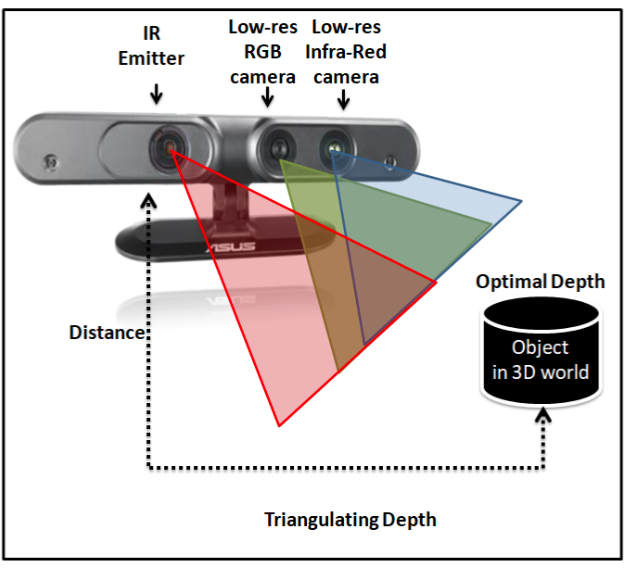
\includegraphics[width=\textwidth]{./images/rgbd-camera-ref.png}
        \label{fig:rgbd}\caption{Funktionsweise RGB-D Kamera\cite[vgl. ][Abbildung 7]{SWB-165930377X}}
    \end{figure}
    
    Da die Geschwindigkeit des Lichts konstant ist, kann die Entfernung zwischen Kamera und Objekt durch Messung der Flugzeit des Lichtstrahls berechnet werden.
    Die Zeit, die das Licht vom Sender zum Empfänger benötigt, wird gemessen und als 'Laufzeit' bezeichnet.
    Die Entfernung berechnet sich nach der gleichen Formel \ref{math:distance} wie auch beim Laser-Entfernungsmesser. 


    Bei \ac{RGB-D} Kameras handelt es sich um Kameras, die ein Strukturlichtverfahren verwenden.
    Bei einem Strukturlichtverfahren werden Lichtmuster auf das zu rekonstruierende Projekt projiziert um das zusätzlich aufgenommene RGB Bild mit Tiefeninformationen zu versehen. Das in Kapitel \ref{chp:lasersensor} verwendete Prinzip wird auf das gesamte Bild angewendet. 
    
    Mithilfe der so gewonnenen Entfernungsinformationen wird eine Tiefenkarte erstellt, die eine 3D Rekonstruktion der Umgebung ermöglicht.

    
    
   Infrarot-Tiefenkameras können auch Farbinformationen aufnehmen, indem sie eine RGB-Kamera in das System integrieren. Durch die Kombination der Tiefenkarte mit der Farbinformation entsteht ein \ac{RGB-D}-Bild, das die Form und die Farbe des Objekts in Echtzeit darstellt.

    Um eine Infrarot-Tiefenkamera in ein System zur Positionsbestimmung oder Umgebungserfassung einzubinden, müssen sowohl die intrinsischen als auch die extrinsischen Parameter bekannt sein. Die intrinsischen Parameter beschreiben die Eigenschaften der Kamera selbst, wie zum Beispiel die Brennweite oder die Verzerrungen, die durch die Linse entstehen. Die extrinsischen Parameter beschreiben die Beziehung zwischen der Kamera und dem Objekt oder der Umgebung, in der sie sich befindet. Hierzu gehören der Abstand, die Ausrichtung und die Position der Kamera im Raum.

    Die Kenntnis beider Parameter ist unerlässlich, um die Tiefenkarte und das RGB-Bild präzise miteinander zu verknüpfen und eine genaue 3D-Rekonstruktion der Umgebung zu erstellen. Die extrinsischen Parameter können durch Kalibrierung der Kamera relativ einfach ermittelt werden, indem bekannte Referenzobjekte im Raum angepeilt werden und die Positionen in der Tiefenkarte und im RGB-Bild verglichen werden. Die intrinsischen Parameter hingegen müssen oft aufwändiger bestimmt werden, beispielsweise durch Analyse von Mustern auf einer Kalibrierungsplatte.
    
    Insgesamt sind Infrarot-Tiefenkameras aufgrund ihrer Fähigkeit zur Erstellung von 3D-Punktwolken und zur gleichzeitigen Erfassung von Farbinformationen eine wertvolle Komponente in verschiedenen Anwendungen wie Robotik, Augmented Reality oder autonomen Fahrzeugen. 

    \cite[vgl.][Kapitel 3]{digital2030022}
    \cite[vgl.]{8310200}
\subsection{Vergleich}\label{chp:depth-sensor-compar}
    Infrarot-Tiefenkameras (\ac{RGB-D}-Kameras) und Laser-Entfernungsmesser finden auch Anwendung im Bereich der Drohnentechnologie.

Infrarot-Tiefenkameras können beispielsweise in Drohnen eingesetzt werden, um eine präzise Hinderniserkennung und -vermeidung zu ermöglichen. Die Kameras können die räumliche Tiefe von Objekten erfassen und somit eine zuverlässige Entfernungsmessung durchführen. Damit kann die Drohne selbstständig Hindernisse erkennen und ausweichen, was insbesondere in unübersichtlichem Gelände oder in der Indoor-Navigation von Vorteil ist.

ToF-Messungen haben in der Regel eine größere Blickfeldbreite als Laser Entfernungsmessungen, was bedeutet, dass sie ein größeres Sichtfeld abdecken können. Dies liegt daran, dass ToF-Messungen Infrarotlicht verwenden, das breiter streut als Laserlicht. Dadurch können ToF-Sensoren größere Bereiche in einem einzigen Messvorgang abdecken und somit mehr Inhalte aufnehmen.

Darüber hinaus haben ToF-Sensoren in der Regel auch eine höhere Bildrate als Laser-Entfernungsmesser. Dies bedeutet, dass sie schneller und kontinuierlicher messen können, was für Anwendungen wie Bewegungserkennung und -verfolgung nützlich sein kann.

Laser-Entfernungsmesser werden häufig eingesetzt, um präzise Entfernungen zu messen, wie beispielsweise bei der Vermessung von Land oder Gebäuden. In der Drohnentechnologie können Laser-Entfernungsmesser eingesetzt werden, um präzise Landungen und Abflüge durchzuführen oder um die exakte Position der Drohne zu bestimmen.




\section{ROS - Robot Operating System} \label{ros:section}
In den vergangenen Jahren hat die Wissenschaft im Bereich der Robotik enorme Fortschritte gemacht. Die Verfügbarkeit zuverlässiger und kostengünstiger Roboterhardware, angefangen bei mobilen Bodenrobotern über Quadrotor-Hubschrauber bis hin zu humanoiden Robotern, ist heute größer als jemals zuvor. Noch beeindruckender ist jedoch die Tatsache, dass Algorithmen entwickelt wurden, die diesen Robotern einen immer höheren Grad an Autonomie verleihen.

Trotz dieser rasanten Fortschritte stehen Softwareentwickler jedoch noch immer vor großen Herausforderungen bei der Programmierung von Robotern. Die Komplexität der Aufgaben, die von Robotern ausgeführt werden können, erfordert eine Menge an spezialisiertem Wissen und Erfahrung in verschiedenen Bereichen wie Sensorik, Bildverarbeitung, Künstlicher Intelligenz und Robotik.

Die Ingenieure und Softwareentwickler haben jedoch die Herausforderungen erkannt und arbeiten intensiv daran, sie zu lösen. Neue Werkzeuge und Frameworks werden entwickelt, um Entwicklern zu helfen, Roboter schneller und effektiver zu programmieren. Eines der bekanntesten Tools in diesem Bereich ist das Robot Operating System \ac{ROS}

\ac{ROS} ist eine Open-Source-Plattform, die speziell für die Entwicklung von Robotersoftware entwickelt wurde. Es bietet eine Reihe von Bibliotheken, Tools und Frameworks, die es Entwicklern ermöglichen, komplexe Robotikanwendungen zu erstellen und zu betreiben. \ac{ROS} wurde von Willow Garage entwickelt und ist heute ein weit verbreitetes Framework in der Robotik-Community.

\ac{ROS} besteht aus verschiedenen Modulen, die es ermöglichen, Roboterhard-  und software zu abstrahieren und zu standardisieren. Die Plattform bietet eine Vielzahl von Werkzeugen für die Entwicklung von Robotik-Software, einschließlich Visualisierungstools, Datenverarbeitungs- und Analysetools sowie eine umfassende Dokumentation.

\ac{ROS} ist so konzipiert, dass es auf einer Vielzahl von Betriebssystemen und Hardwarearchitekturen laufen kann und bietet Unterstützung für eine breite Palette von Robotern und Sensoren. Es ist auch bekannt für seine Fähigkeit zur Zusammenarbeit zwischen verschiedenen Robotern, die miteinander kommunizieren und Aufgaben gemeinsam erledigen können.

Dank seiner leistungsstarken Funktionen und Flexibilität ist \ac{ROS} zu einem der wichtigsten Frameworks für die Robotik-Entwicklung geworden und wird in vielen Anwendungen eingesetzt, von industriellen Robotern bis hin zu autonomen Fahrzeugen. \cite[vgl.][]{ROSIntroduction}

    \subsection{Vorraussetzungen zur Verwendung von ROS} \label{Vorraussetzungen zur Verwendung von ROS:subsection}
    Die verschiedenen \ac{ROS} Versionen setzen bestimmte \ac{OS} Versionen voraus. Am besten funktioniert hierbei Linux und hierbei Ubuntu. Aber auch auf Mac OS kann man ROS verwenden. Allerdings ist die Version für Mac OS bislange nur experimentell. \ac{ROS} funktioniert auch unter Windows allerdings werden nicht alle Pakete unterstützt \cite[vgl.][]{ROSIntroduction}.

    \subsection{ROS-Distributionen} \label{ROS-Distributionen:subsection}
    Eine ROS-Distribution besteht aus einem festgelegten und visionierten Set von ROS-Paketen. Vergleichbar ist dieses System mit den Linux-Distributionen wie z.B. Ubuntu. Der Hauptzweck von ROS-Distributionen besteht darin, Entwicklern eine relativ stabile Codebasis zu bieten, damit sie daran weiterarbeiten können. Sobald eine Distribution veröffentlicht wurde, werden Änderungen hauptsächlich auf Fehlerbehebungen und nicht-zerstörerische Verbesserungen für die Kernpakete (alles unter ros-desktop-full) beschränkt. Somit ist das 'Umziehen' auf eine neue Distribution weniger fehleranfällig und einfacher. Dies gilt im Allgemeinen für die gesamte ROS-Community, jedoch sind die Regeln für 'höhere' Pakete weniger streng und somit liegt es an den Verantwortlichen eines spezifischen Pakets, zerstörende Änderungen zu vermeiden \cite[vgl.][]{ROScontributions}.

    \subsection{Nodes} \label{nodes:subsection}
    In \ac{ROS} werden Funktionen und Prozesse durch sogenannte Nodes realisiert. Eine Node ist eine ausführbare Einheit, die in einem \ac{ROS}-System arbeitet und über eine eindeutige Identifikation verfügt. Jede Node hat eine spezifische Aufgabe, wie beispielsweise das Sammeln von Sensordaten, die Ausführung einer spezifischen Berechnung oder das Steuern eines Aktors.

    Nodes können miteinander kommunizieren, indem sie Nachrichten senden und empfangen. Nachrichten sind definierte Datenstrukturen, die Informationen zwischen Nodes transportieren. Nodes können auch Services anbieten oder anfordern, um eine bestimmte Aktion auszuführen.

    Eine wichtige Funktion von Nodes ist ihre Fähigkeit zur Verteilung. In \ac{ROS} können Nodes auf verschiedenen Hosts oder in verschiedenen Prozessen ausgeführt werden. Dadurch können komplexe \ac{ROS}-Systeme erstellt werden, die aus vielen miteinander verbundenen Nodes bestehen.

    Nodes können auch in einer \ac{ROS}-Graphenstruktur organisiert werden. Diese Struktur zeigt die Abhängigkeiten zwischen Nodes und die Art der Kommunikation zwischen ihnen an. Die \ac{ROS}-Graphenstruktur kann mit Werkzeugen wie "rqt\_graph" visualisiert werden, um eine bessere Übersicht über das System zu erhalten.

    Die Verwendung von Nodes in \ac{ROS} ermöglicht eine hohe Flexibilität und Modularität bei der Entwicklung von Robotik-Anwendungen. Entwickler können einzelne Nodes erstellen, testen und optimieren, bevor sie sie in einem größeren System einsetzen. Darüber hinaus können Nodes wiederverwendet werden, um ähnliche Funktionen in verschiedenen Anwendungen auszuführen.

    Insgesamt sind Nodes eine zentrale Komponente von \ac{ROS} und ermöglichen es Entwicklern, komplexe Roboteranwendungen mit einer hohen Flexibilität und Modularität zu erstellen.
    \cite[vgl.][]{ROSNodes}


    \subsection{Topics} \label{topics:subsection}
    In \ac{ROS} werden Daten zwischen Nodes durch sogenannte Topics ausgetauscht. Ein Topic ist eine benannte Kommunikationsleitung, über die Nodes Nachrichten senden und empfangen können. Topics ermöglichen die einfache und flexible Kommunikation zwischen Nodes, ohne dass die Nodes über die genaue Identität des Empfängers Bescheid wissen müssen.

    Ein Topic hat einen bestimmten Datentyp, der definiert, welche Art von Daten zwischen Nodes ausgetauscht werden können. Es können beispielsweise Sensordaten wie Bilder oder Entfernungsmessungen, oder Steuerbefehle für Aktoren wie Motoren oder Greifer übertragen werden.

    Nodes können sich auf ein Topic abonnieren, um die Nachrichten, die auf diesem Topic veröffentlicht werden, zu empfangen. Jedes Mal, wenn eine Nachricht auf einem Topic veröffentlicht wird, wird sie an alle Nodes weitergeleitet, die auf dieses Topic abonniert sind.

    Topics können auch von Nodes veröffentlicht werden, um Nachrichten an andere Nodes zu senden. Eine Node, die ein Topic veröffentlicht, wird als Publisher bezeichnet. Der Publisher kann regelmäßig Nachrichten auf einem Topic veröffentlichen, um andere Nodes über Änderungen in der Umgebung oder im System zu informieren.

    Die Verwendung von Topics in \ac{ROS} ermöglicht eine einfache und flexible Kommunikation zwischen Nodes, was besonders in komplexen Systemen von Vorteil ist. Nodes können sich auf mehrere Topics abonnieren und Nachrichten an mehrere Topics veröffentlichen, was eine effektive und modulare Datenverarbeitung ermöglicht. Zudem können Topics auf mehreren Hosts oder in verschiedenen Prozessen ausgeführt werden, was eine Skalierung des \ac{ROS}-Systems ermöglicht.

    Insgesamt sind Topics eine wichtige Komponente von \ac{ROS} und ermöglichen es Entwicklern, eine einfache und effektive Kommunikation zwischen Nodes in Robotik-Anwendungen zu realisieren. \cite[vgl.][]{ROSTopics}

    \subsection{Messages} \label{messages:subsection}
    Die Messages sind Datenströme, die zwischen mindestens zwei Nodes ausgetauscht werden. Sie werden in sogenannten msg-Dateien definiert. Diese Nachrichten können sowohl aus primitiven Datentypen als auch aus Datenstrukturen bestehen. Der Datenfluss erfolgt immer nur in eine Richtung. \cite[vgl.][]{ROSMessages}

    \subsection{Publish and Subscripe Pattern} \label{publish_and_subscripe_pattern:subsection}
    Das Publish-Subscribe-Pattern ist ein grundlegendes Muster der \ac{ROS}-Kommunikation und ermöglicht eine effektive und modulare Datenverarbeitung in verteilten Systemen.

    Beim Publish-Subscribe-Pattern senden Nodes, die Informationen über eine bestimmte Ressource verarbeiten, die Informationen an ein Topic, das als Vermittler dient. Nodes, die an den Informationen interessiert sind, abonnieren das Topic und erhalten alle zukünftigen Nachrichten, die von Nodes veröffentlicht werden, die mit dem Topic verbunden sind.

    Dieses Muster hat mehrere Vorteile. Zum einen ermöglicht es eine flexible Architektur, in der Nodes unabhängig voneinander arbeiten und sich auf das Abonnieren und Veröffentlichen von Topics konzentrieren können, ohne die genaue Identität des Empfängers oder Senders zu kennen. Zum anderen ermöglicht es eine effektive Datenverarbeitung, da mehrere Nodes dieselben Informationen von einem Publisher erhalten können.

    Ein weiterer Vorteil des Publish-Subscribe-Patterns ist, dass es eine einfache Möglichkeit bietet, den Zustand von Ressourcen zu überwachen oder auf Änderungen in Echtzeit zu reagieren. So kann beispielsweise eine Node, die eine Kamera überwacht, die Bilder auf einem Topic veröffentlichen. Andere Nodes, die an der Verarbeitung dieser Bilder beteiligt sind, können sich auf das Topic abonnieren und die Informationen in Echtzeit verarbeiten.

    Das Publish-Subscribe-Pattern ist ein grundlegendes Konzept in \ac{ROS} und wird in der Regel für die Kommunikation zwischen Nodes verwendet. Es ermöglicht eine effektive und modulare Datenverarbeitung in verteilten Systemen und ist ein wesentlicher Bestandteil von \ac{ROS}, um komplexe Robotik-Anwendungen zu realisieren.
    
    \cite[vgl.][]{ROSconcepts}

\section{MAVLink} \label{mavlink}
\ac{MAVLink} ist ein Nachrichtenprotokoll, welches vor allem zur Kommunikation zwischen einer Drohne und einer Bodenstation eingesetzt wird. Der Einsatz dieses Protokolls ist besonders für Systeme konzipiert, die wenige Ressourcen und eine geringe Bandbreite aufweisen.\\
Die Kommunikation kann über verschiedene Wege stattfinden, hierzu gehören beispielsweise \ac{USB}, aber auch drahtlose Verbindungen über Wifi, mit \ac{UDP} sowie auch \ac{TCP}, sind möglich. Das Protokoll überträgt Telemetriedaten mit Hilfe des Publisher/Subscriber Modells. Protokolle die Änderungen an der Systemkofiguration bewirken, wie beispielsweise ein Parameter- oder auch ein Missionsprotokoll und dadurch eine garantierte Zustellung erfordern, werden hingegen Punkt-zu-Punkt mit Retransmission übertragen. 

Der Sender so wie der Empfänger der Nachricht haben jeweils eine einzigartige ID, sodass sie nachvollziehen können, von dem die Nachricht geschickt wurde. Sobald eine Verbindung zwischen der Station und der Drohne besteht, senden sich die zwei Systeme gegenseitig in bestimmten Abständen einen sogenannten Heartbeat, um sicherzustellen, dass die Verbindung noch besteht.
Benötigt die Bodenstation Telemetriedaten der Drohne, so sendet die Station eine Anfrage an die Drohne, welche daraufhin die angeforderten Daten sendet. \cite{mavlink}

\begin{figure}[H]
    \begin{centering}
        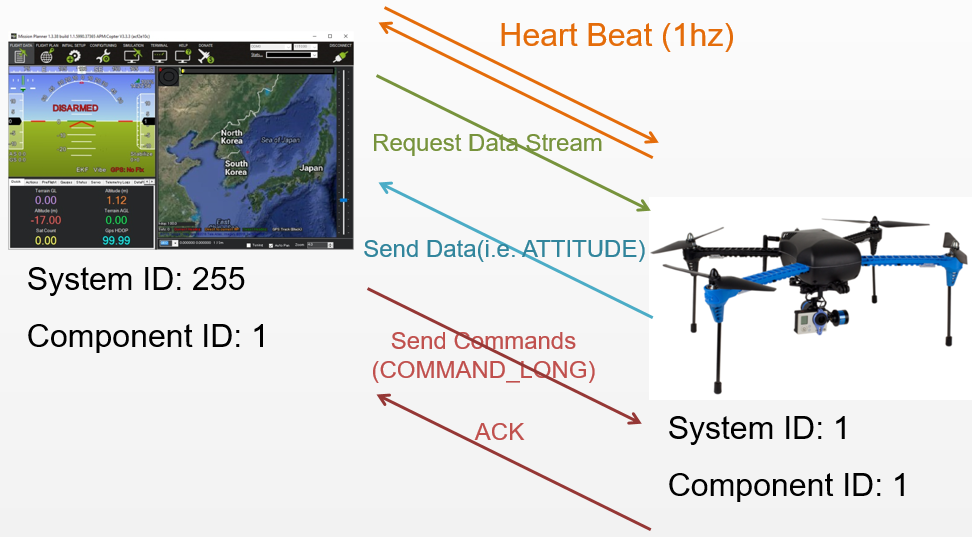
\includegraphics[scale=0.4]{images/mavlink-message-flow.png}
        \caption{\label{img mavlink}Nachrichten MAVLink \cite{imgmavlink}}
    \end{centering}
\end{figure}


\section{Multicopter} \label{drohne:section}

Multicopter, auch als \ac{UAV}s bekannt, repräsentieren eine aufstrebende Technologie mit vielfältigen Anwendungsmöglichkeiten. Besonders hervorzuheben ist die Überwachung und Kartierung schwer zugänglicher Gebiete. Durch den Einsatz hochauflösender Kameras und Sensoren können Drohnen präzise Bilder und Daten liefern, die zur Kartenerstellung und Beobachtung von Flora und Fauna genutzt werden.

Die Inspektion von Infrastrukturen wie Brücken, Windkraftanlagen und Pipelines stellt einen weiteren wichtigen Einsatzbereich dar. Durch ihre Fähigkeit, schnell und effizient in schwer zugängliche Bereiche zu fliegen, ermöglichen Drohnen visuelle Inspektionen ohne die physische Präsenz eines Inspektors. Dadurch kann die Inspektionszeit erheblich reduziert und die Sicherheit der Inspektoren verbessert werden.

Drohnen bieten auch eine innovative Möglichkeit zur Warenlieferung, insbesondere in Gebieten mit eingeschränkter Infrastruktur. Einige Unternehmen experimentieren bereits mit Drohnenlieferungen, und dieser Anwendungsbereich wird voraussichtlich in Zukunft weiter wachsen.

Trotz dieser vielfältigen Anwendungsmöglichkeiten ist es entscheidend, geeignete regulatorische Rahmenbedingungen und technologische Verbesserungen sicherzustellen, um einen sicheren und effektiven Einsatz von Drohnen zu gewährleisten.


Das Herzstück des Regelungssystems ist der Flightcontroller, der in der Lage ist, Sensordaten zu verarbeiten und die Steuerung des Multicopters anzupassen, um eine stabile Fluglage und präzise Positionierung zu gewährleisten. Die in einem Flightcontroller verwendeten Steuerungsalgorithmen sind häufig komplex und umfassen oft eine Kombination aus Proportional-Integral-Derivative (PID)-Reglern und anderen Regelungstechniken.
Bei der Entwicklung und dem Betrieb von Multikoptern sind eine Reihe von wichtigen Überlegungen anzustellen. Eine davon ist die Batterielebensdauer und Energieeffizienz der Drohne, die weitgehend durch das Energiemanagement und die Batteriekapazität bestimmt wird. Fortschritte in der Batterietechnologie und energieeffiziente Komponenten können die Flugzeiten erheblich verlängern und die Drohne in die Lage versetzen, längere Einsätze zu fliegen oder schwerere Nutzlasten zu transportieren.

Ein entscheidender Aspekt des Multikopterbetriebs sind die Kommunikations- und Steuersysteme, die Informationen zwischen der Drohne und dem Bediener übermitteln. Dazu können Funkfrequenzsteuerungen, GPS-Systeme für die Navigation und möglicherweise Mobilfunk- oder Satellitenkommunikation für Einsätze über große Entfernungen oder außerhalb der Sichtlinie gehören.

Je nach Verwendungszweck des Multikopters kann er mit verschiedenen Sensoren und Zubehörteilen ausgestattet werden. Dazu können hochauflösende Kameras, LiDAR, Wärmebildkameras, Greifer oder Sprühgeräte gehören. Durch diese Anpassungen können Drohnen für bestimmte Aufgaben wie Luftaufnahmen, Infrastrukturinspektionen, landwirtschaftliche Überwachung oder Lieferaufgaben maßgeschneidert werden.

Sicherheit ist beim Drohnenbetrieb von größter Bedeutung, und Multicopter verfügen häufig über mehrere Sicherheitsmechanismen. Dazu gehören Funktionen zur Rückkehr nach Hause bei Verlust des Steuersignals, Kollisionsvermeidungssysteme zur Vermeidung von Abstürzen und Notlandeverfahren, wenn eine kritische Störung festgestellt wird. Auch Redundanz in kritischen Systemen wie Motoren und Steuerungen kann die Sicherheit der Drohne insgesamt erhöhen.

Schließlich kann die Leistung und Steuerung eines Multikopters durch Wetter- und Umweltbedingungen erheblich beeinträchtigt werden. Drohnen müssen so konstruiert sein, dass sie den Bedingungen standhalten, unter denen sie eingesetzt werden, und die Piloten müssen wissen, wie sich diese Bedingungen auf die Flugeigenschaften auswirken können. Dazu gehört, dass man versteht, wie Wind die Stabilität und Steuerung beeinflussen kann, wie die Temperatur die Batterieleistung beeinträchtigen kann und wie Niederschlag den Sensorbetrieb beeinflusst. Daher sind Wetter- und Umwelteinflüsse ein wichtiger Bestandteil des Betriebs und der Konstruktion von Multikoptern.

\cite[vgl.][UAV Fundamentals]{Valavanis2015}
\subsection{Aufbau Quadrocopter}

Quadrocopter sind eine bestimmte Art von Multicoptern, die mit vier Rotoren ausgestattet sind. Diese Rotoren sind in der Regel in einer quadratischen oder rechteckigen Konfiguration angeordnet, und die Bewegung des Quadrocopters wird durch die Änderung der Geschwindigkeit und Richtung dieser Rotoren gesteuert.

Der Schlüssel zum Betrieb eines Quadrocopters ist das Gleichgewicht und die Steuerung der vier Rotoren. Jeder Rotor erzeugt sowohl Auftrieb als auch Drehmoment. Damit der Quadrocopter während des Fluges stabil bleibt, muss das Drehmoment das den Quadrocopter ins Trudeln bringt würde ausgeglichen werden. Wie in \ref{fig:frames} zu sehen müssen die gegebüberliegenden Rotoren dafür in gegensätzliche Richtungen drehen um das Drehmoment auszugleichen.

Die Steuersysteme von Quadrocoptern verwenden in der Regel PID-Regler (Proportional, Integral, Derivativ). Diese Regler passen die Drehzahl der Rotoren auf der Grundlage der Differenz zwischen der gewünschten und der tatsächlichen Position oder Ausrichtung des Quadrocopters an, beschrieben werden sie in \ref{chp:pid}.

\cite[vgl.][Quadrocopter Kinematic and Dynamics]{Valavanis2015}

\begin{figure}
    \begin{centering}
        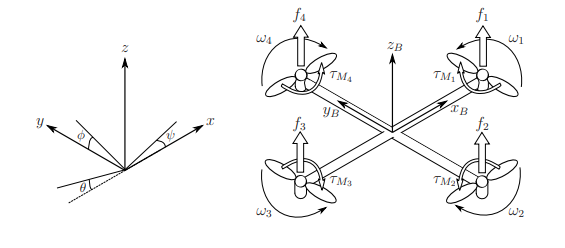
\includegraphics[scale=0.6]{images/inertial_body_frames.png}
        \caption{\label{fig:frames}Rotationskraefte vgl. \cite{luukkonen2011modelling}}
    \end{centering}
\end{figure}


\subsection{Freiheitsgrade}

Ein Quadrocopter besitzt 6 Freiheitsgrade, genauso wie Flugzeuge. Sie haben jedoch andere Möglichkeiten diese Freiheitsgrade zu nutzen.
Quadrocopter können jedoch im Gegensatz zu Flugzeugen direkt mit diesen Freiheitsgraden navigieren. In \ref{fig:freiheitsgrade} sehen Sie ein Schaubild der Freiheitsgrade.
Folgende Freiheitsgrade kann ein Quadrocopter verwenden.

\begin{description}
    \item[Pitch] Der Pitch-Freiheitsgrad gibt an, ob sich der Multicopter nach vorne oder nach hinten neigt. Wenn der Copter nach vorne geneigt ist, beschleunigt er nach vorne, wenn er nach hinten geneigt ist, bremst er ab. Der Pitch wird durch unterschiedliche Drehzahlen der Rotoren auf der Vorder- und Hinterseite des Multicopters gesteuert.
    \item[Yaw] Der Yaw-Freiheitsgrad gibt an, ob sich der Multicopter um die Hochachse dreht. Eine Veränderung des Yaw-Freiheitsgrads erfolgt durch unterschiedliche Drehzahlen der Rotoren auf gegenüberliegenden Seiten des Multicopters. Dies ermöglicht dem Multicopter, seine Ausrichtung im Raum zu ändern und zu drehen.
    \item[Roll] Der Roll-Freiheitsgrad gibt an, ob sich der Multicopter nach links oder rechts neigt. Eine Neigung nach rechts führt zu einer Beschleunigung in diese Richtung, während eine Neigung nach links eine Verzögerung oder Bremsung bewirkt. Der Roll wird durch unterschiedliche Drehzahlen der Rotoren auf der linken und rechten Seite des Multicopters gesteuert.
    \item[Sideslip] Der Sideslip-Freiheitsgrad gibt an, ob sich der Multicopter seitlich bewegt, ohne dabei zu rollen oder zu neigen. Eine Bewegung in eine Richtung führt zu einem Drift in diese Richtung. Der Sideslip kann durch unterschiedliche Drehzahlen der Rotoren auf gegenüberliegenden Seiten des Multicopters gesteuert werden.
    \item[Tilt] Der Tilt-Freiheitsgrad bezieht sich auf die Fähigkeit des Multicopters, sich um eine Achse zu drehen, die zwischen den Rotoren verläuft. Dies ermöglicht dem Multicopter, sich in eine bestimmte Richtung zu neigen und seine Ausrichtung im Raum zu ändern.
    \item[Lift] Der Lift-Freiheitsgrad bezieht sich auf die Fähigkeit des Multicopters, vertikal zu steigen oder zu sinken. Der Lift wird durch die Änderung der Drehzahlen aller Rotoren gleichzeitig gesteuert.    
\end{description}

\begin{figure}[H]
\begin{centering}
    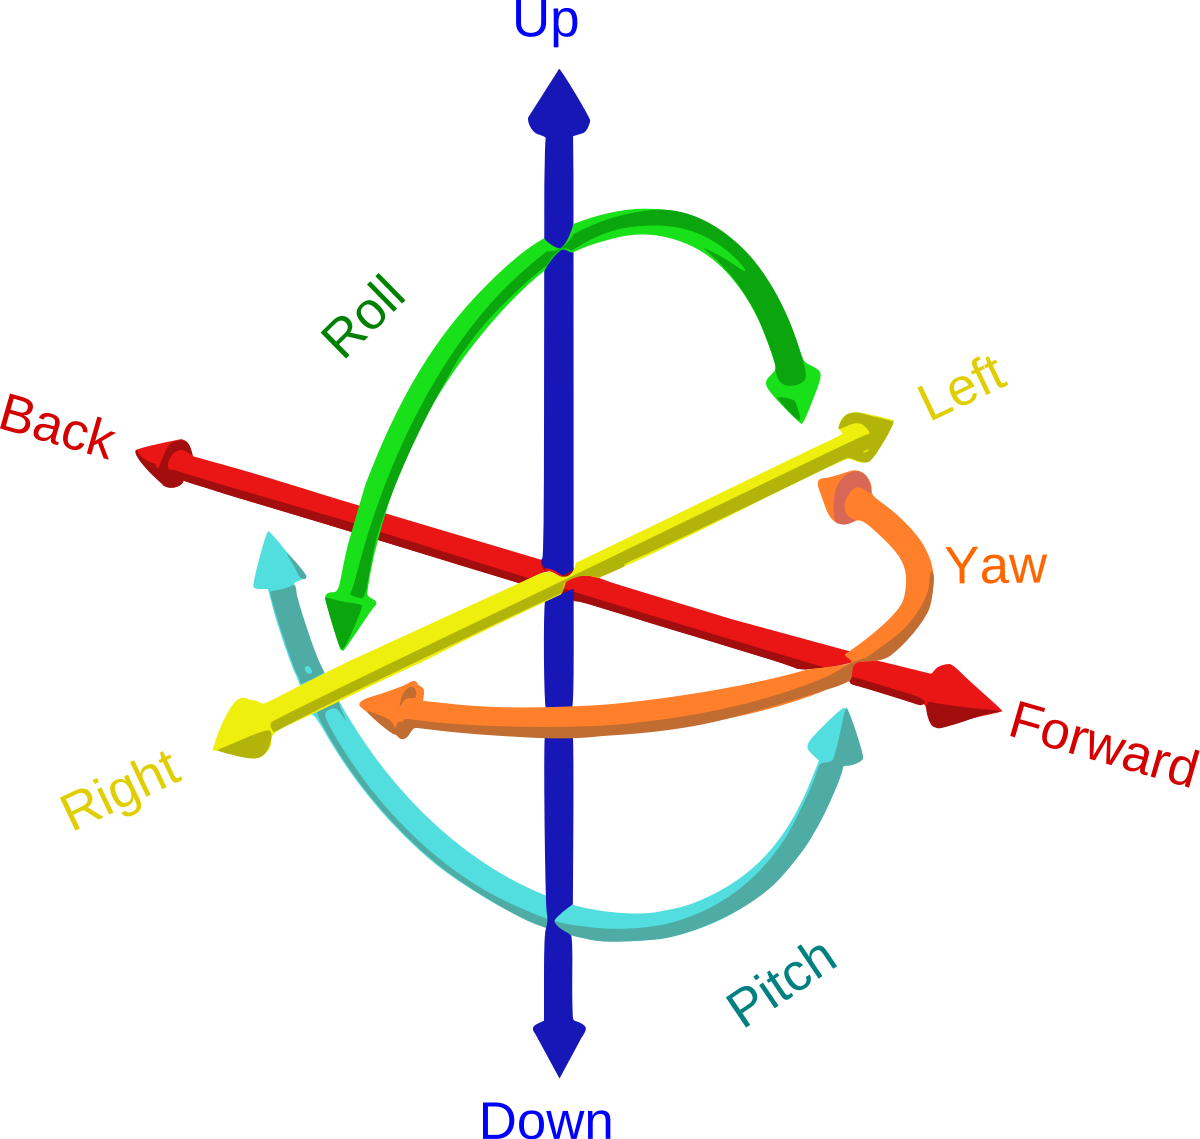
\includegraphics[scale=0.2]{images/multicopter_freiheitsgrade.png}
    
    \caption{\label{fig:freiheitsgrade}Multicopter Freiheitsgrade \cite{imgfreiheitsgrade}}
\end{centering}
\end{figure}
    
\cite[vgl.][Kapitel 5]{SWB-165930377X}




\section{Regelsysteme} \label{regelsysteme:section}


    \subsection{P-Regler}
    \label{chp:p-regler}
    
    Ein \ac{P-Regler} ist eine grundlegende Form der Regelungstechnik, die oft in industriellen Anwendungen verwendet wird. Der \ac{P-Regler} basiert auf dem Prinzip der proportionalen Rückkopplung. Er wirkt, indem der Regler die Differenz zwischen dem Ist- und Sollwert signalisiert und dann eine proportionale Regelgröße zum Fehler signalisiert.
    Es gibt eine direkte proportionale Beziehung zwischen der Ausgangsleistung des Reglers und dem Fehler. Die mathematische Formel für den P-Regler ist: 

    \begin{figure}[H]
    \begin{equation*}
        u(t) = K_p e(t)
    \end{equation*}
    \eqlabel{eq:p-regler}{P-Regler}

\end{figure}

    wo $u(t)$ das Signal des Reglers, $K_p$ der Proportionalitätsfaktor und $e(t)$ der Fehler zwischen der Ist- und Sollwert der Regelgrößen ist.

    \subsection{I-Regler}
\label{chp:i-regler}

    Neben \ac{P-Regler}n gibt es \ac{I-Regler}.
    Aus dem Name \ac{I-Regler}, lässt sich das Wort \textit{Integral} ableiten. Ein \ac{I-Regler} ist eine Form der Regelungstechnik, die verwendet wird, um den Regelgrößenfehler zwischen Soll- und Istwert zu minimieren und das System auf den Sollwert zu bringen. 

    Der I-Regler basiert auf dem Prinzip der Integration des Regelgrößenfehlers über die Zeit. Die mathematische Gleichung für den I-Regler ist:

    \begin{figure}[H]
        \begin{equation*}
            u(t) = K_i \int_{0}^{t} e(\tau) d\tau
        \end{equation*}
        \eqlabel{eq:i-regler}{I-Regler}
    \end{figure}

    wo $u(t)$ das Signal des Reglers, $K_i$ der Integrationsfaktor und $e(t)$ der Regelgrößenfehler ist. Der Integrationsfaktor ist ein Maß für die Empfindlichkeit des Reglers auf den Regelgrößenfehler.

Durch einen höheren $K_i$ Faktor reagiert der Regler stärker, führt jedoch auch zu langsameren Reaktionszeiten des Reglers.

    Das \ac{I-Regler} summiert Regeldifferenzen auf, dies resultiert darin, dass die Regeldifferenz im geschlossenen Regelkreis gegen den Wert 0 läuft.



    \subsection{D-Regler}
    \label{chp:d-regler}
    
    Ein weiterer wichtiger Regler ist der \ac{D-Regler}. Ein \ac{D-Regler} wird verwendet um den Regelgrößefehler zwischen Soll- und Istwert zu minimieren.

    Der \ac{D-Regler} wird verwendet, um das System zu stabilisieren und auf Störungen zu reagieren. Die mathematische Gleichung für den D-Regler lautet:

    \begin{figure}[H]
        \begin{equation*}
            u(t) = K_d \frac{de(t)}{dt}
        \end{equation*}
        \eqlabel{eq:d-regler}{D-Regler}
    \end{figure}


    \subsection{PID-Regler} \label{chp:pid}
    Ein PID-Regler ist ein häufig verwendeter Reglertyp in der Regelungstechnik. Die Abkürzung PID steht für Proportional-Integral-Derivative, was die drei Hauptkomponenten des Reglers beschreibt. Der proportionale Teil des Reglers reagiert proportional zur Abweichung zwischen der gemessenen Prozessgröße und dem gewünschten Wert, der integrale Teil berücksichtigt die vergangene Abweichung und der derivative Teil reagiert auf die Geschwindigkeit, mit der sich die Abweichung ändert.

    Eine genauere Beschreibung der einzelnen Regelglieder finden Sie in den Kapiteln: 
    \begin{itemize}
        \item{P-Glied \ref{chp:p-regler}}
        \item{I-Glied \ref{chp:i-regler}}
        \item{D-Glied \ref{chp:d-regler}}
    \end{itemize}


Die Kombination dieser drei Komponenten ermöglicht es dem PID-Regler, schnell auf Veränderungen des Prozesses zu reagieren und gleichzeitig stabile Regelungsergebnisse zu erzielen. Die Einstellung der Reglerparameter, wie z.B. des Proportionalitätsfaktors, des Integrationszeitraums und des Differentiationszeitraums, ist jedoch eine wichtige Herausforderung bei der Anwendung von PID-Reglern.

PID-Regler finden in vielen Anwendungen Anwendung, einschließlich Temperaturregelung, Geschwindigkeitsregelung, Positionierung und Flugzeugsteuerung.
\cite[vgl. ][Kapitel 11.3]{SWB-165930377X}


   
\subsection{Flightstack}

Der Flightstack eines Multicopters besteht aus mehreren Systemen. Üblicherweise besteht der Flightstack aus Mikrocontrollern, Sensoren, Aktuatoren, GPS-Modul und einer Stromversorgung. Die Sensoren sind dafür zuständig Daten über die aktuelle Fluglage des Multicopters zu sammeln. Daten die gesammelt werden, sind Beschleunigung, Neigung, Lage und GPS-Position. Diese Daten werden vom Mikrocontroller verarbeitet, um die Steuerung der Aktuatoren zu optimieren. Im Outdoor Flug ermöglicht die Verwendung eines GPS-Moduls die Position des Multicopters zu bestimmen und zu verfolgen.

Da die verbaute Technik auch mit Strom versorgt werden muss, ist ein Akkumulator auf dem Multicopter verbaut. Der Akkumulator stellt die nötige Energie für den Betrieb des Multicopters bereit. Insgesamt ist der Flightstack ein zentrales Element zur Steuerung des Multicopters und erfordert eine sorgfältige Integration und Abstimmung aller Komponenten, um eine zuverlässige und sichere Steuerung zu gewährleisten.

\cite[vgl.][Kapitel 2.4.2]{SWB-165930377X}

\section{3D-Modelle} \label{3d-modelle:section}
3D-Modelle sind digitale Nachbildungen von physischen Objekten oder Szenen in drei Dimensionen. Diese Modelle werden in verschiedenen Branchen und Anwendungen eingesetzt, von der Architektur und Ingenieurwesen über Film und Gaming bis hin zur Medizin und dem Design von Produkten.

Die Erstellung von 3D-Modellen erfolgt in der Regel durch eine Kombination von verschiedenen Technologien und Software-Tools. Zum Beispiel können 3D-Scanner verwendet werden, um physische Objekte zu scannen und daraus digitale Modelle zu erstellen. Alternativ können 3D-Modelle auch von Grund auf neu erstellt werden, indem man eine 2D-Zeichnung oder ein Konzept in einer 3D-Software modelliert.

Ein wichtiger Vorteil von 3D-Modellen ist, dass sie interaktiv und manipulierbar sind. Das bedeutet, dass man sie drehen, skalieren und animieren kann, um verschiedene Perspektiven oder Bewegungen zu erzeugen. Darüber hinaus können 3D-Modelle auch für Simulationen und Analysen verwendet werden. Zum Beispiel können Architekten und Ingenieure 3D-Modelle von Gebäuden erstellen, um die Belastung bei Erdbeben oder starkem Wind zu simulieren.

Insgesamt sind 3D-Modelle eine äußerst vielseitige Technologie, die in vielen verschiedenen Branchen und Anwendungen eingesetzt werden kann. Sie ermöglichen es, physische Objekte und Szenen digital darzustellen und zu manipulieren, was zahlreiche Möglichkeiten für Design, Simulation und Analyse bietet.

\subsection{3D-Scanner}
Ein 3D-Scanner ist ein Gerät, das Objekte oder Umgebungen erfasst und digitale 3D-Modelle erstellt. Im Gegensatz zu einem herkömmlichen Scanner, der nur flache Bilder erzeugt, kann ein 3D-Scanner eine vollständige dreidimensionale Darstellung eines Objekts erstellen.

Es gibt verschiedene Arten von 3D-Scannern, darunter Laserscanner, strukturiertes Licht, Fotogrammetrie und Time-of-Flight-Scanner. Jeder dieser Scanner verwendet unterschiedliche Technologien und Methoden zur Erfassung von Daten.

Laserscanner verwenden Laserlicht, um die Form eines Objekts zu erfassen, während strukturiertes Licht eine Reihe von Mustern projiziert, um die Oberfläche eines Objekts zu messen. Fotogrammetrie nutzt Bilder, die von verschiedenen Blickwinkeln aufgenommen werden, um ein 3D-Modell zu erstellen, während Time-of-Flight-Scanner die Zeit messen, die benötigt wird, um einen Lichtpuls zu reflektieren, um Entfernungen zu messen.

Die Verwendung von 3D-Scannern ist in vielen Branchen und Anwendungen weit verbreitet, einschließlich Reverse Engineering, Architektur, Medizin, Unterhaltung, Kunst und Design. 3D-Scanner ermöglichen es den Benutzern, genaue Messungen von Objekten zu erhalten, die in der realen Welt existieren, und diese in digitale Formate zu konvertieren, die leichter zu bearbeiten und zu teilen sind.

Es gibt auch mobile 3D-Scanner, die in Handys und Tablets integriert sind, und diese ermöglichen es Benutzern, schnell und einfach 3D-Modelle von Objekten zu erstellen, ohne dass zusätzliche Geräte erforderlich sind.

Obwohl 3D-Scanner ein unglaublich leistungsfähiges Werkzeug sind, haben sie auch einige Einschränkungen. Zum Beispiel können sie Schwierigkeiten haben, sehr dunkle oder glänzende Objekte genau zu erfassen. Trotzdem sind 3D-Scanner ein wertvolles Instrument für jeden, der in der Lage sein möchte, genaue 3D-Modelle von Objekten oder Räumen zu erstellen und sie in digitale Formate zu konvertieren.

\subsubsection{Lasertriangulation}
Bei der Lasertriangulation wird ein Laserstrahl wird an der Oberfläche des Messobjektes reflektiert und über eine Optik und einen Umlenkspiegel auf eine lichtempfindliche Zeilenkamera projiziert. Abhängig von der Entfernung des Messobjektes verändert sich die Position des Lichtpunktes. Hieraus ermittelt der Signalprozessor den Abstand zwischen dem Sensor und der Oberfläche der Stahlprodukte. \cite[vgl.][]{Lasertriangulation}

\subsubsection{3D-Scanner mit strukturiertem Licht}
Scanner für strukturiertes Licht verwenden ebenfalls die trigonometrische Triangulation. Allerdings verwenden sie keinen Laser. Das System projiziert eine Reihe an linienförmigen Mustern of auf Objekt. Zum Erkennen des Abstandes werden die Kanten jeder Linie des Musters untersucht. Anhand dieser Kanten kann dann der Abstand vom Scanner zum Objekt berechnet werden. Im Wesentlichen „sieht“ die Kamera nicht eine Laserlinie, sondern den Rand des projizierten Musters. \cite[vgl.][]{strukturiertsLicht}

\subsubsection{Time-of-flight-Scanner}
Time-of-Flight (ToF) Scanner sind eine Art von 3D-Scanner, die mithilfe von Lichtimpulsen die Entfernung zu Objekten in Echtzeit messen können. Sie haben in den letzten Jahren aufgrund ihrer hohen Genauigkeit und ihrer Fähigkeit, schnelle und präzise Messungen durchzuführen, eine breite Anwendung in verschiedenen Branchen gefunden.

ToF-Scanner verwenden in der Regel eine Kombination aus Infrarot-Licht und Kameras, um Tiefeninformationen zu sammeln. Der Scanner sendet einen kurzen Lichtimpuls aus und misst dann die Zeit, die benötigt wird, um zum Objekt zurückzukehren. Durch die Messung der Zeit und die Analyse des reflektierten Lichts kann der Scanner die Entfernung zum Objekt bestimmen und daraus ein 3D-Modell des Objekts erstellen. \cite[vgl.][]{TOF}

\subsubsection{Laser-Phasenverschiebungs-Scanner}
Laser-Phasenverschiebungs-Scanner arbeiten auf eine sehr ähnliche Art wie die Time-of-flight-Scanner. Der Scanner verwendet nicht nur die Zeit, die der Laser braucht, sondern wertet auch seine Phasenverschiebung, welche auf dem Weg vom Senden und Empfangen entsteht, aus.

Der Laserstrahl wird auf das Objekt gerichtet und reflektiert zurück zur Kamera. Das reflektierte Licht enthält Informationen über die Form des Objekts, die durch die Phasenverschiebung des Lichts bestimmt werden kann. Die Phasenverschiebung wird gemessen, indem der Laserstrahl in unterschiedlichen Winkeln auf das Objekt gerichtet wird, was zu unterschiedlichen Phasenverschiebungen führt. Die Kamera nimmt Bilder des reflektierten Lichts auf und die Phasenverschiebung der reflektierten Lichtwellen wird berechnet. Diese Informationen werden dann verwendet, um ein 3D-Modell des Objekts zu erstellen.

Der Scanner vergleicht die Phase des Aussendens des Lasers mit der Rückführung des Lasers zum Sensor. Die Messung der Phasenverschiebung ist eine präzisere Methode.

\subsection{Tiefenkammera}
Eine Tiefenkamera ist eine Art von Kamera, die mithilfe von verschiedenen Technologien wie beispielsweise Stereovision oder Time-of-Flight (ToF) die Entfernung von Objekten im Bild ermitteln kann.

Bei der Stereovision werden zwei Kameras verwendet, die jeweils dasselbe Objekt aus einer etwas anderen Perspektive betrachten. Durch die Analyse der Unterschiede in den beiden Bildern kann die Tiefenkamera die Entfernung zu den Objekten im Bild bestimmen.

Die Time-of-Flight-Technologie verwendet dagegen einen Laser oder eine LED, um Lichtimpulse auf die Umgebung zu senden und die Zeit zu messen, die benötigt wird, um vom Objekt zurückzukehren. Je länger das Licht braucht, um zurückzukehren, desto weiter entfernt ist das Objekt. Diese Technologie ermöglicht es der Tiefenkamera, die Entfernung zu Objekten in Echtzeit zu messen und sogar Bewegungen in Echtzeit zu verfolgen.

Die erfassten Tiefendaten können dann verwendet werden, um beispielsweise 3D-Modelle von Objekten oder Umgebungen zu erstellen. \cite[vgl.][]{TiefenKamera}

\subsection{Punktwolken}
Eine Punktwolke ist eine räumliche Darstellung eines Objekts oder einer Szene in Form einer Sammlung von 3D-Koordinaten. Am Beispiel von \ac{RGB-D} Kameras erfasst eine Punktwolke sowohl Farb- als auch Tiefeninformationen aus einer Szene.
Die Tiefeninformationen werden verwendet, um die räumliche Geometrie der Szene zu erfassen und eine Punktwolke zu erstellen.
Die Punktwolke besteht aus einer Sammlung von Punkten, die jeweils eine Position im dreidimensionalen Raum repräsentieren. Jeder Punkt hat in der Regel drei Koordinaten (x, y, z), die seine Position im Raum beschreiben. Die Farbinformationen werden häufig als RGB-Werte (rot, grün, blau) oder als Grauwerte für jeden Punkt in der Punktwolke gespeichert.
Eine \ac{RGB-D}-Kamera erfasst die Tiefeninformationen durch die Verwendung eines Strukturlichtverfahrens oder eines Zeitflugverfahrens. Strukturlichtverfahren arbeiten durch die Projektion von Lichtmuster auf die Szene und das Erfassen der Verzerrungen im Muster, um die Tiefeninformationen zu berechnen. Zeitflugverfahren funktionieren durch die Messung der Zeit, die benötigt wird, um ein Lichtsignal auszusenden und das reflektierte Signal wieder zu empfangen, um die Entfernung und damit die Tiefeninformationen zu berechnen.

Die erfasste Punktwolke wird dann für verschiedene Anwendungen verwendet, wie z.B. für die Erstellung von 3D-Modellen, für die Positionsbestimmung von Robotern oder für die Objekterkennung in der Robotik. Da die Punktwolken alle Informationen über die räumliche Geometrie einer Szene enthalten, sind sie ein wichtiges Instrument für viele Anwendungen in der Robotik, der Computer Vision und der Augmented Reality.


\section{Positionsbestimmung und Kartenerstellung}
\label{positionsbestimmung:section}
Positionsbestimmung ist ein wichtiges Thema in vielen Bereichen, wie der Robotik, autonomem Fahren, Navigation und Augmented Reality. Eine der Herausforderungen bei der Positionsbestimmung ist die Erstellung einer genauen Karte der Umgebung, die es dem mobilen Gerät ermöglicht, seine Position darin zu bestimmen. Hier kommen Technologien wie \ac{SLAM} (Simultaneous Localization and Mapping) und Spatial Mapping zum Einsatz. Beide Ansätze ermöglichen die Erstellung von 3D-Karten der Umgebung, aber sie unterscheiden sich in ihren Methoden und Anwendungen. In dieser Hinsicht sind \ac{SLAM} und Spatial Mapping wichtige Technologien für die Positionsbestimmung und haben eine breite Anwendung in verschiedenen Branchen gefunden.

\subsection{Koordinatensysteme}

Eine Drohne, die im dreidimensionalen Raum navigiert und visuelles \ac{SLAM} verwendet, arbeitet mit mehreren Koordinatensystemen, zwischen denen Transformationen durchgeführt werden müssen. Insbesondere visuelles \ac{SLAM} wird oft mit Inertial- oder IMU-Daten kombiniert, um genaue und robuste Positionsschätzungen zu erhalten.

Für eine Drohne, die im dreidimensionalen Raum navigiert, können die folgenden Koordinatensysteme definiert werden:

\begin{description}
    \item[Weltkoordinatensystem]{Dieses Koordinatensystem stellt die absolute Position und Orientierung der Drohne in Bezug auf die Umgebung dar. Es wird in der Regel als globales Referenzsystem betrachtet und kann z. B. mit \ac{GPS}-Koordinaten oder einem festen Startpunkt definiert werden.}
    \item[Lokales Koordinatensystem]{Dieses Koordinatensystem wird normalerweise in Verbindung mit visuellem \ac{SLAM} verwendet und dient der Beschreibung der relativen Bewegungen und Positionen von Merkmalen oder Punkten in der Umgebung der Drohne. Es kann sich z. B. auf einen bestimmten Hauptpunkt oder ein Merkmal beziehen, das als Referenzpunkt für die Positionsbestimmung verwendet wird.}
    \item[Kamerakoordinatensystem]{
        Dieses Koordinatensystem ist mit der Kamera der Drohne verbunden und bewegt sich mit ihr. Es wird verwendet, um die Position und Ausrichtung von Punkten im Kamerabild zu beschreiben. In der Regel wird das Kamerakoordinatensystem so definiert, dass die optische Achse der Kamera die Z-Achse bildet und die X- und Y-Achsen in der Bildebene liegen.} 
    \item[\ac{IMU} Koordinatensystem]{Eine Inertialmesseinheit (IMU) in der Drohne misst Beschleunigung und Winkelgeschwindigkeit. Das IMU-Koordinatensystem ist mit der IMU verbunden und bewegt sich mit ihr. Es ist normalerweise so definiert, dass die Z-Achse senkrecht zur Erdanziehung ausgerichtet ist und die X- und Y-Achse entsprechend eingestellt sind.} 
    \item[Navigatioskoordinatensystem]{Ein Navigationskoordinatensystem ist ein spezielles Koordinatensystem, das für die Navigation verwendet wird. Es kann in verschiedenen Kontexten definiert werden, aber im Allgemeinen bezieht es sich auf ein Koordinatensystem, das speziell dazu dient, die Position und Ausrichtung von Objekten (wie Schiffen, Flugzeugen oder Drohnen) in Bezug auf die Erdoberfläche zu bestimmen. In der Robotik oder in autonomen Fahrzeugen bezieht es sich meist auf ein lokales Koordinatensystem, das die relative Position und Ausrichtung des Roboters oder Fahrzeugs in Bezug auf seine unmittelbare Umgebung beschreibt.} 
\end{description}


Während der Navigation und Lokalisierung kombiniert die Drohne Informationen aus diesen verschiedenen Koordinatensystemen, um genaue Positionsschätzungen zu erhalten. Die Transformationen zwischen den Koordinatensystemen werden unter Berücksichtigung der kinematischen Eigenschaften der Drohne und der Sensorinformationen berechnet, um die genaue Position und Ausrichtung der Drohne im Raum zu bestimmen.


    \cite[vgl. ]{SWB-1841134112}

 \subsection{Extended Kalman Filter 2}
    Der \ac{EKF}2-Algorithmus, der in der Drohnensteuerung verwendet wird, ist eine Erweiterung des klassischen erweiterten Kalman-Filters, die speziell auf die Bedürfnisse der Drohnensteuerung zugeschnitten ist. Der EKF2 ist ein geschätzter Zustandsregler, der die aktuellen Zustände (z.B. Position, Geschwindigkeit, Orientierung) einer Drohne schätzt, basierend auf Messungen von Sensoren (z.B. \ac{GPS}, \ac{IMU}, Magnetometer).

Im Gegensatz zum klassischen EKF verwendet der EKF2 eine modifizierte Version der Kalman-Filter-Formeln, um den Einfluss von Sensorrauschen und Messfehlern besser zu berücksichtigen. Insbesondere verwendet der EKF2 eine sogenannte 'Innovation Covariance Matrix', die die Varianz der Messfehler repräsentiert und in die Filtergleichungen eingebaut wird. Diese Innovation Covariance Matrix wird iterativ während des Betriebs des Filters aktualisiert, um Sensorrauschen und Messfehlern besser gerecht zu werden.

Darüber hinaus verwendet der EKF2 eine modifizierte Version der State Transition Matrix, die die Nichtlinearitäten des Systems besser modellieren kann. Diese modifizierte Matrix wird ebenfalls iterativ während des Filterbetriebs aktualisiert, um den Änderungen im Systemverhalten besser gerecht zu werden.

In der Drohnensteuerung wird der EKF2-Algorithmus verwendet, um die aktuellen Zustände der Drohne (z.B. Position, Geschwindigkeit, Orientierung) in Echtzeit zu schätzen. Diese Schätzungen werden dann verwendet, um die Steuerbefehle der Drohne zu generieren, um sie auf Kurs zu halten und sicher zu navigieren.
    
    \subsection{Spatial Mapping} \label{spatial_mapping:subsection}

    Spatial Mapping hingegen ist ein Prozess, bei dem eine 3D-Karte der Umgebung auf der Grundlage der Verarbeitung von Kameradaten erstellt wird. Im Gegensatz zum \ac{SLAM}-Prozess muss das mobile Gerät, das die 3D-Karte erstellt, seine Position in der Umgebung bereits kennen, da es auf der Verarbeitung von Kameradaten basiert. Die Kameras nehmen Bilder auf und wandeln sie in 3D-Punktwolken um, die dann zu einer Karte kombiniert werden. Spatial Mapping wird in Augmented-Reality-Anwendungen und anderen Anwendungen eingesetzt, bei denen eine genaue 3D-Karte der Umgebung benötigt wird.
    Spatial Mapping hat jedoch einige Einschränkungen.
    Es ist schwierig eine genaue Karte zu erstellen, wenn sich das mobile Gerät schnell bewegt oder die Umgebung stark verändert. Außerdem ist die Anwendungsbreite von Spatial Mapping auf Anwendungen beschränkt, bei denen eine genaue Karte ausreichend ist, ohne das eine kontinuierliche Positionsschätzung erforderlich ist.
   
    \subsection{Inertielle Positionsbestimmung} \label{inertielle_positionsbestimmung:subsection}
    Inertiale Positionsbestimmung ist ein weiterer Ansatz zur Positionsbestimmung, der auf der Verwendung von Inertialsensoren wie Gyroskopen und Beschleunigungsmessern basiert. Inertialsensoren messen die Veränderungen der Beschleunigung und der Winkelgeschwindigkeit eines mobilen Geräts, was dazu verwendet werden kann, die Position und Orientierung des Geräts in der Umgebung zu bestimmen. Die Inertiale Positionsbestimmung hat jedoch auch einige Herausforderungen, da die Inertialsensoren anfällig für Driftfehler sind. Diese Fehler können durch die Integration der Beschleunigung und der Winkelgeschwindigkeit über die Zeit entstehen und zu Ungenauigkeiten bei der Positionsbestimmung führen. Um diesen Fehler zu korrigieren können Inertialsensoren mit anderen Sensoren wie Magnetometern oder GPS kombiniert werden.
    Eine andere Möglichkeit besteht darin, die Inertialsensor-Daten in einen \ac{SLAM}- oder Spatial Mapping-Prozess zu integrieren, um eine genauere Positionsbestimmung zu erzielen. Durch die Kombination von Inertialsensor-DAten mit visuellen DAten können die Vorteile beider Ansätze genutzt werden und die Nachteile minimiert werden.


Allerdings ist die inertielle Positionsbestimmung anfällig für Fehler, die aufgrund von Drift und Ungenauigkeiten der Inertialsensoren entstehen können. Um diese Fehler zu minimieren, wird die inertielle Positionsbestimmung oft mit anderen Technologien wie GPS oder visuellen Systemen kombiniert. Diese Kombination von Technologien wird auch als Sensorfusion bezeichnet und ermöglicht eine präzisere und robustere Positionsbestimmung in verschiedenen Anwendungen wie Drohnen, autonomen Fahrzeugen und Wearables.

\section{SLAM}\label{SLAM:section} 

Der \ac{SLAM}-Prozess umfasst die simultane Bestimmung der Position eines mobilen Geräts in der Umgebung und die Erstellung einer Karte dieser Umgebung. Dies wird durch die Integration von Daten aus verschiedenen Sensoren wie Kameras, Inertialsensoren und Entfernungsmessern wie Laser-Scannern oder Time-of-Flight-Sensoren erreicht. Der \ac{SLAM}-Prozess wird oft in der Robotik und in autonomen Fahrzeugen eingesetzt, um eine präzise Karte der Umgebung zu erstellen und sich gleichzeitig darin zu lokalisieren.
Durch die Kombination der Inertialsensoren mit anderen Sensoren kann eine präzisere und robustere Positionsbestimmung erreicht werden, indem die Vorteile der verschiedenen Technologien kombiniert werden. Die Inertialsensoren können beispielsweise verwendet werden, um die Bewegung des mobilen Geräts zwischen den einzelnen Beobachtungen durch die anderen Sensoren zu messen und die Positions- und Orientierungsdaten der \ac{SLAM}-Systeme zu korrigieren.

Da Multicopter sich im dreidimensionalen Raum bewegen werden im Folgenden nur \ac{SLAM} Verfahren betrachtet, die sich im dreidimensionalen Raum befinden.

\subsection{Anforderungen an \ac{SLAM} Systeme auf Multicoptern}

\begin{description}
    \item[Echtzeitfähigkeit]{Da Multikopter in dynamischen Umgebungen operieren und schnell auf Veränderungen reagieren müssen, ist die Echtzeitfähigkeit des \ac{SLAM}-Algorithmus entscheidend. Um genaue und aktuelle Informationen zu liefern, muss der SLAM-Algorithmus in der Lage sein, die Daten in Echtzeit zu verarbeiten. Auf diese Weise kann der Multikopter die Umgebung ständig genau wahrnehmen und sicher navigieren.}
    \item[Effizienz]{
        Effizienz ist ein wichtiger Faktor für den \ac{SLAM}-Algorithmus in Multicoptern, da Ressourcen wie Rechenleistung und Batteriekapazität begrenzt sind. Effiziente SLAM-Algorithmen minimieren den Ressourcenverbrauch durch den Einsatz optimierter Datenverarbeitungstechniken und Algorithmen. Dadurch wird sichergestellt, dass der Multikopter über längere Zeiträume autonom arbeiten kann, ohne dass die Ressourcen schnell erschöpft sind.}
    \item[Genauigkeit]{Die Genauigkeit des \ac{SLAM}-Algorithmus wirkt sich direkt auf die Qualität der erstellten Karte und die genaue Lokalisierung des Multikopters aus. Durch die Kombination von Daten aus verschiedenen Sensoren und die Anwendung fortschrittlicher Algorithmen zur Erkennung und Verfolgung von Merkmalen wird eine höhere Genauigkeit erreicht. Dank der präzisen Wahrnehmung und Lokalisierung kann der Multikopter zuverlässig navigieren und Hindernissen in der Umgebung ausweichen.}
    \item[Robustheit]{Der SLAM-Algorithmus muss robust gegenüber Umgebungsbedingungen, Sensorrauschen und unvorhergesehenen Ereignissen sein, um eine zuverlässige Leistung in verschiedenen Situationen zu gewährleisten. Robuste \ac{SLAM}-Methoden können Rauschen filtern, sensorbedingte Fehler korrigieren und ungenaue Messungen erkennen und berücksichtigen. So bleibt der Multicopter auch in schwierigen Umgebungen stabil und einsatzfähig.}
    \item[Skalierbarkeit]{Die Skalierbarkeit des \ac{SLAM}-Algorithmus ermöglicht seinen Einsatz auf verschiedenen Plattformen und in unterschiedlichen Umgebungen. Ein skalierbarer SLAM-Algorithmus kann sich an unterschiedliche Sensorkonfigurationen, Multikoptermodelle und Umgebungen anpassen. Dadurch wird sichergestellt, dass der \ac{SLAM}-Algorithmus auf Multikoptern mit unterschiedlichen Hardwarekapazitäten und -anforderungen effektiv eingesetzt werden kann.}
    \item[3D Kartenerstellung]{Die Fähigkeit zur 3D Kartenerstellung ermöglicht eine detaillierte und umfassende Repräsentation der Umgebung für den Multicopter. Durch die Integration von Daten aus 3D-Sensoren wie Lidar können hochauflösende Punktwolken erstellt werden, die eine präzise Darstellung der räumlichen Struktur bieten. Eine genaue 3D Kartenerstellung ermöglicht dem Multicopter eine genauere Navigation, Hindernisvermeidung und eine bessere Interaktion mit der Umgebung.} 
\end{description}

Zusammenfassend ist es entscheidend, dass der \ac{SLAM}-Algorithmus in Multikoptern Echtzeitfähigkeit, Effizienz, Genauigkeit, Robustheit, Skalierbarkeit und 3D-Mapping bietet. Wenn diese Anforderungen erfüllt sind, kann der Multikopter autonom in dynamischen Umgebungen navigieren, Hindernissen ausweichen und genaue Karten der Umgebung erstellen. Die kontinuierliche Entwicklung von \ac{SLAM}-Algorithmen in diesen Bereichen ermöglicht fortschrittlichere und zuverlässigere Multikopter-Anwendungen in verschiedenen Szenarien.

\subsection{Datenaquirierung}

Die Datenerfassung umfasst die Erfassung von Informationen von verschiedenen Sensoren, die am Multikopter angebracht sind, wie z. B. Kameras, Lidar und Trägheitsmessgeräte (IMUs). Diese Sensoren liefern verschiedene Arten von Daten, die für \ac{SLAM} unerlässlich sind. Kameras erfassen visuelle Bilder der Umgebung und ermöglichen die Erkennung und Verfolgung von Merkmalen, was in visuellen \ac{SLAM}-Algorithmen häufig verwendet wird. Lidar-Sensoren hingegen senden Laserstrahlen aus, um Entfernungen zu Objekten zu messen, und liefern präzise 3D-Punktwolkendaten. \ac{IMU}s helfen bei der Erfassung der Orientierung, Beschleunigung und Winkelgeschwindigkeit des Multicopters.

\begin{description}
    \item[Kameras] Kameras werden bei Multicopter-\ac{SLAM} in großem Umfang zur visuellen Datenerfassung eingesetzt. Sie erfassen Bilder der Umgebung, die anschließend für die Erkennung und Verfolgung von Merkmalen verarbeitet werden. Kamerabasierte \ac{SLAM}-Algorithmen extrahieren visuelle Merkmale, wie z. B. Ecken oder Eckpunkte, und verfolgen sie über die Zeit, um die Position und Ausrichtung des Multikopters zu schätzen. Allerdings kann die Genauigkeit der kamerabasierten Datenerfassung durch Probleme wie Verdeckungen, Beleuchtungsschwankungen und Bildrauschen beeinträchtigt werden.
    Eine besondere Kamera ist die \ac{RGB-D} Kamera, sie kombiniert einen Tiefensensor mit einer normalen Kamera.
    \item[Lidar]Lidar-Sensoren liefern präzise Tiefeninformationen, indem sie Laserstrahlen aussenden und die Zeit messen, die die Strahlen benötigen, um zurückzukehren. Dies ermöglicht die Erzeugung von 3D-Punktwolken, die für die Umgebungskartierung bei Multicopter-\ac{SLAM} von unschätzbarem Wert sind. Die Lidar-basierte Datenerfassung bietet Vorteile wie Robustheit gegenüber Lichtverhältnissen und die Fähigkeit, feinkörnige geometrische Details zu erfassen. Dennoch müssen Herausforderungen wie ein begrenztes Sichtfeld, Sensorinterferenzen und Rechenanforderungen für eine effektive Integration von Lidar-Daten in SLAM-Systeme berücksichtigt werden.
    \item[IMUs]IMUs bestehen aus Beschleunigungsmessern und Gyroskopen, die die lineare Beschleunigung bzw. die Winkelgeschwindigkeit messen. Diese Sensoren liefern wichtige Bewegungsinformationen für das \ac{SLAM} von Multikoptern, indem sie Änderungen der Fluglage des Multikopters im Laufe der Zeit schätzen. IMUs tragen zur Vorhersage und Korrektur der Flugbahn des Multikopters während der Kartierungs- und Lokalisierungsprozesse bei. Allerdings können inhärentes Sensorrauschen und Drift die Genauigkeit der IMU-Daten beeinträchtigen, so dass Kalibrierungs- und Fusionstechniken für eine optimale Nutzung erforderlich sind.  
\end{description}


\subsection{Extrinsische und Intrinsische Kameraparameter}

Die intrinsische Kameraparemter ist eine 3x3 Matrix, siehe \ref{eq:intrinsic-matrix} und beschreibt die Abbildungseigenschaften der Kamera und enthält Informationen wie Brennweite, Verschiebung und Verzerrung. Um diese Matrix zu erhalten, werden Kalibrierungsbilder von der Kamera aufgenommen und anschließend eine Kalibrierungssoftware verwendet, um die intrinsischen Parameter der Kamera zu berechnen. Die intrinsischen Parameter bleiben konstant, solange die Kamera nicht verändert wird, beispielsweise durch Zoomen oder Fokussieren. Daher müssen sie nur einmal ermittelt werden, solange die Kameraeinstellungen gleich bleiben. Diese Parameter sind wesentlich für die korrekte Interpretation und Verarbeitung der von der Kamera erfassten Bilder, da sie es ermöglichen, eine Verbindung zwischen den Pixelkoordinaten im Bild und den tatsächlichen Positionen im Raum herzustellen.

 \begin{itemize}
    \item $f_x$ und $f_y$ sind die Brennweiten in Pixeln, entsprechend den X- und Y-Achsen.
    \item $c_x$ und $c_y$ sind die Koordinaten des Hauptpunkts
    \item $s$ ist ein zusätzlicher Scherungsparameter
 \end{itemize}

Die extrinsische Matrix ist eine 4x4-Matrix, siehe \ref{eq:extrinsic-matrix} die in homogenen Koordinaten ausgedrückt wird und die Transformation von Kamerakoordinaten in Weltkoordinaten beschreibt. Diese Transformation umfasst die Translation der Kamera und die Rotation um die Achsen des Weltkoordinatensystems. Die extrinsische Matrix wird verwendet, um die 3D-Position jedes Punktes in der Szene relativ zur Kamera zu bestimmen.

Sobald die intrinsische Matrix bekannt ist, kann die extrinsische Matrix bestimmt werden. Diese Matrix beschreibt die Position und Ausrichtung der Kamera im Raum relativ zum Weltkoordinatensystem. Um diese Matrix zu berechnen, werden mehrere Bilder von der Kamera aus verschiedenen Positionen aufgenommen und mithilfe von visuellen Odometrie- oder \ac{SLAM}-Algorithmen verarbeitet, um die Kameraposition und -orientierung zu schätzen.

\begin{figure}
    \begin{equation*}
        K = \begin{bmatrix}
        f_x & s & c_x \\
        0 & f_y & c_Y \\
        0 & 0 & 1
        \end{bmatrix}
        \end{equation*}
        \caption{Intrinsische Matrix für eine \ac{RGB-D} camera}
        %\label{eq :intrinsic-matrix}
        \eqlabel{eq:intrinsic-matrix}{Intrinsische Maxtrix}
    \end{figure}  


    \begin{figure}
        \begin{equation*}
            T_{ext}=\begin{bmatrix}
                r_{11} & r_{12} & r_{13} & t_x\\
                r_{21} & r_{22} & r_{23} & t_y\\
                r_{31} & r_{32} & r_{33} & t_z\\
                0 & 0 & 0 & 1
                \end{bmatrix}   
        \end{equation*}
        \caption{Extrinsische Matrix für eine \ac{RGB-D} Kamera}
        \eqlabel{eq:extrinsic-matrix}{Extrinsische Matrix}
    \end{figure}
    
   \cite[vgl.][Kapitel 1.2]{SWB-1681722674} 

\subsection{Punktwolkentransformation}

Punktwolken sind ein zentraler Bestandteil von 3D-Modellen und werden in verschiedenen Anwendungen wie 3D-Rekonstruktion, Objekterkennung und Augmented Reality eingesetzt. Sie stellen eine dreidimensionale Repräsentation der realen Welt dar und bestehen aus einer großen Anzahl von Punkten, die die räumliche Struktur und Form der Objekte in der Szene beschreiben.

Ein Punktwolkengenerator erzeugt eine Punktwolke aus mehreren Bildern, die von einer Kamera aufgenommen wurden.

Um die Punktwolke zu erzeugen müssen 2D Koordinaten in ein 3D Koordinatensystem überführt werden, dazu benötigt man zunächst die intrinsische und die extrinsische Matrix der Kamera. 

In Kombination mit der intrinsischen Matrix ermöglicht die extrinsische Matrix die Umwandlung von 2D-Bildpunkten in korrekte 3D-Objektpunkte. Die intrinsischen Parameter beschreiben die Abbildungseigenschaften der Kamera und die extrinsischen Parameter beschreiben die Position und Orientierung der Kamera relativ zum Weltkoordinatensystem. Zusammen ermöglichen sie die genaue Rückprojektion von 2D-Bildpunkten in den 3D-Raum und somit die Erzeugung einer genauen Punktwolke. 

Die Transformationsmatrix, die die Transformation von Kamerakoordinaten in Weltkoordinaten beschreibt, kann aus der intrinsischen Matrix und der extrinsischen Matrix berechnet werden. Die Formel finden Sie in \ref{eq:transform-matrix}

\cite{SWB-470983582}

\begin{figure}[H]
\begin{equation*}
T = K \begin{bmatrix}R & t\end{bmatrix}
\end{equation*}
\eqlabel{eq:transform-matrix}{Transformationsmatix}
wobei $K$ die intrinsische Matrix, $R$ die 3x3 Rotationsmatrix aus der extrinsischen Matrix und $t$ der 3x1 Translationsvektor aus der extrinsischen Matrix ist. Das Symbol $\begin{bmatrix}R & t\end{bmatrix}$ bezeichnet die erweiterte Matrix, die aus der Kombination von $R$ und $t$ gebildet wird.
\end{figure}

Durch Wiederholung dieses Prozesses für jedes 2D-Bild wird eine Punktwolke erzeugt, die eine dreidimensionale Repräsentation der Szene darstellt. Ein wichtiger Aspekt bei der Erstellung einer Punktwolke ist es, dass die Bilder aus verschiedenen Blickwinkeln aufgenommen werden. Dadurch kann eine größere Menge an Information über die Szene erfasst werden, was zu einer genaueren und detaillierteren Punktwolke führt.

Dieser Prozess entspricht dem Pinhole Kamera Modell, in Abbildung \ref{fig:3dtransformation} ist es bildlich dargestellt.

\begin{figure}
    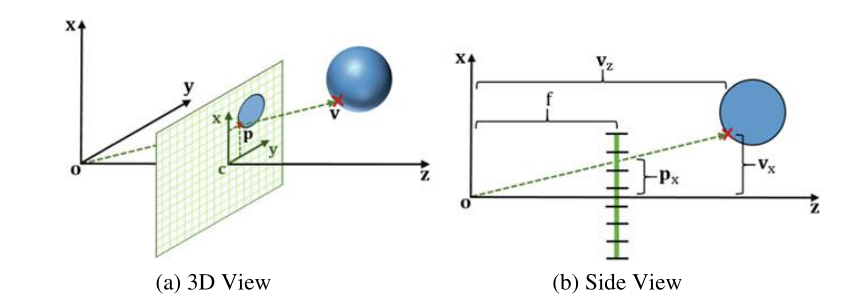
\includegraphics[width=\textwidth]{./images/transformation.png}
    \label{fig:3dtransformation}
    \caption{Das Modell der Pinhole-Kamera
    Modell beschreibt, wie ein Punkt $v \in R3$ auf eine Stelle $p \in R2$ auf dem Sensor abgebildet wird. Die z-Achse ist die
    Richtung der Kamera und die x-Achse ist der Aufwärtsvektor. Die perspektivische Projektion ist gegeben durch
    die Brennweite der Kamera $f$ und den Hauptpunkt $c$. Die Brennweite $f$ ist der Abstand zwischen der Sensorebene und dem Ursprung o der perspektivischen Projektion.
    der Sensorebene und dem Ursprung o des Kamerakoordinatensystems.\cite[vgl. S.6]{SWB-1681722674}}
\end{figure}

Es ist auch zu beachten, dass bei der Erzeugung von Punktwolken aus \ac{RGB-D}-Bildern eine weitere wichtige Matrix verwendet wird: die Transformationsmatrix. Diese Matrix beschreibt die Beziehung zwischen der Kamera und dem Tiefensensor und ermöglicht es, die 3D-Position jedes Punktes in der Szene basierend auf der Tiefeninformation des Sensors zu bestimmen. Der Prozess in dem diese Beziehung berechnet wird nennt sich Registrierung und umfasst folgende Schritte:

\begin{description}
    \item[1. Transformation in den 3D-Raum:] Zunächst wird das Tiefenbild, das ursprünglich als 2D-Bild mit Tiefenwerten an jedem Pixel dargestellt wird, in eine Punktwolke im 3D-Raum umgewandelt. Dies geschieht unter Verwendung der intrinsischen Parameter der Tiefenkamera und der Tiefenwerte an jedem Pixel.
    
    \item [2. Ausrichtung der Sensoren:] Da die RGB- und Tiefensensoren aus verschiedenen Winkeln auf die Szene schauen, muss eine Transformationsmatrix verwendet werden, um die Punktwolke aus der Perspektive der RGB-Kamera zu betrachten. Diese Transformationsmatrix repräsentiert die extrinsischen Parameter zwischen den beiden Kameras und wird durch Kalibrierung des Systems bestimmt.
    
    \item[3. Projektion auf das RGB-Bild:] Schließlich wird die transformierte Punktwolke auf das 2D-RGB-Bild projiziert, um ein \ac{RGB-D}-Bild zu erstellen. Dies geschieht unter Verwendung der intrinsischen Parameter der RGB-Kamera.
    \end{description}

    \cite[vgl.][Kapitel 5.3.1]{SWB-1681722674}

    


Insgesamt ist die Erzeugung einer Punktwolke ein komplexer Prozess, der sowohl die intrinsischen als auch extrinsischen Parameter der Kamera erfordert. Es erfordert auch die Verarbeitung von mehreren Bildern aus verschiedenen Blickwinkeln und gegebenenfalls die Verwendung von Tiefensensoren. Trotzdem ist die Erzeugung von Punktwolken ein wichtiger Schritt für viele Anwendungen in der Computergrafik und -vision. Zum Beispiel kann die Punktwolke für die Erstellung von 3D-Modellen verwendet werden, um virtuelle Umgebungen für Computerspiele und Simulationen zu erstellen oder für die Erkennung von Objekten und Hindernissen in autonomen Fahrzeugen.

Es gibt viele Algorithmen und Technologien, die für die Erzeugung von Punktwolken verwendet werden können, darunter Stereo-Vision, Structured-Light-Scanning und Time-of-Flight-Sensoren. Jede Methode hat ihre eigenen Vor- und Nachteile, und die Wahl der am besten geeigneten Methode hängt von den Anforderungen der Anwendung ab.

Grundsätzlich geht es aber darum 2D Koordinaten eines Bildes in ein dreidimensionales festes Koordinatengitter zu überführen, das der Realität entspricht.

\cite[vgl.][Kapitel 9.2 und Kapitel 7.8.1]{SWB-165930377X}



\subsection{Visuelle Odometrie \& und visuelles SLAM}

Die Themen \ac{VO} und \ac{VSLAM} sind eng miteinander verknüpft und zielen darauf ab, 3D-Informationen aus visuellen Datenströmen in Echtzeit zu extrahieren. \ac{VO} zielt darauf ab, die inkrementelle Bewegung der Kamera zu schätzen, während \ac{VSLAM} sich darauf konzentriert, eine global konsistente Karte der Szene und die Kameratrajektorie in Bezug darauf zu schätzen.

In der Robotikforschung wird \ac{SLAM} als grundlegende Fähigkeit für autonome Roboter betrachtet. Frühe Arbeiten zu \ac{SLAM} nutzten hauptsächlich Laserscanner, jedoch hat das Feld aufgrund von Fortschritten in der Computer Vision und verbesserter Prozessoren schnell auf Kameras umgestellt.

Mit Visueller Odometrie kann die Bewegung der Drohne geschätzt werden, so können auch Hindernisse im Flugfeld der Drohne erkannt werden.

\subsection{Herausforderungen und Lösungen in Visueller Odometrie und VSLAM}

Die meisten visuellen \ac{SLAM}-Methoden basieren auf Merkmalsabgleich und Mehransichtsgeometrie. Dies bringt einige Herausforderungen und Einschränkungen mit sich, insbesondere für monokulare SLAM. Zu diesen Herausforderungen gehören die Notwendigkeit einer großen Basislinienbewegung, um ausreichend Parallaxe für eine zuverlässige Tiefenschätzung zu erzeugen, und die Unbeobachtbarkeit der Skala. Diese Probleme können teilweise durch den Einsatz zusätzlicher Sensoren, wie Stereo-Kameras und Trägheitsmesseinheiten (\ac{IMU}s), oder durch Vorwissen über das System oder die Szene gelöst werden. Ein weiteres Problem ist die dichte Rekonstruktion von Bereichen mit geringer Textur.

Da in dieser Kamera eine \ac{RGB-D} Kamera verwendet wird, die das monokulare Bild der RGB Kamera mit Tiefeninformationen versorgt, werden monokulare \ac{SLAM} Verfahren in dieser Arbeit nicht betrachtet. Es werden nur \ac{SLAM} Verfahren betrachtet, die direkt mit \ac{RGB-D} Kameras umgehen können.

Bei \ac{SLAM} Verfahren, die neben den visuellen Datenströmen noch Daten von einer \ac{IMU} verwenden können, spricht man von Visual Inertial \ac{SLAM}.

\subsubsection{Loop Closure}

Dies ist ein entscheidendes Konzept bei \ac{SLAM}, das sich auf das Problem bezieht, einen Ort zu erkennen, den der Roboter oder das Fahrzeug zuvor besucht hat, um die aufgelaufenen Lokalisierungsfehler zu korrigieren. Im Kontext von \ac{VSLAM} beinhaltet der Schleifenschluss den Abgleich einer aktuellen Ansicht mit einer früheren Ansicht, wodurch festgestellt wird, dass das System zu einem zuvor besuchten Ort zurückgekehrt ist. Dieser Vorgang ist für die Aufrechterhaltung der Genauigkeit der Karte von entscheidender Bedeutung, da er es dem System ermöglicht, die im Laufe der Zeit auftretende Abweichung zu korrigieren.

Methoden zur Erkennung von Schleifenschlüssen können in lokale, globale und segmentbasierte Methoden unterteilt werden. Lokale Deskriptormethoden verwenden häufig Punktverteilungsinformationen zur Beschreibung von Merkmalen. Diese lokalen Merkmale sind jedoch möglicherweise nicht aussagekräftig genug, um ähnliche lokale Strukturen zu unterscheiden. Globale Deskriptoren hingegen werden aus dem gesamten Sensorscan, z. B. einem LiDAR-Scan, generiert und können eine Konvertierung der 3D-Punktwolke in eine 2D-Bilddarstellung erfordern. Diese Methoden reagieren in der Regel empfindlich auf Änderungen des Blickwinkels und den teilweisen Verlust von Punkten. In jüngerer Zeit wurden segmentierungsbasierte Ansätze vorgeschlagen, bei denen Punktwolken in verschiedene Elemente segmentiert, ihre Merkmale extrahiert und die entsprechenden Elemente abgeglichen werden. Diese Ansätze arbeiten auf semantischer oder objektbezogener Ebene und sind oft robuster gegenüber Verdeckungen und anderen Umgebungsvariablen.

\subsubsection{Trajektorien}

Die Flugbahn eines Roboters oder Fahrzeugs bezieht sich auf seinen Weg durch die Umgebung. Im Kontext von \ac{SLAM} ist die Trajektorie die Abfolge von Posen (Positionen und Ausrichtungen), die der Roboter oder das Fahrzeug im Laufe der Zeit einnimmt. ORB-SLAM berechnet beispielsweise die Kameratrajektorie in Echtzeit und liefert eine zeitliche Abfolge von Kamerapositionen, die für Navigation, Bewegungsanalyse und Szenenrekonstruktion verwendet werden können.

\subsubsection{Surfel Repräsentation}

Im Kontext der 3D-Kartierung und -Visualisierung ist ein Surfel, kurz für "Oberflächenelement", eine Datenstruktur, die zur Darstellung eines kleinen Teils einer Oberfläche im 3D-Raum verwendet wird. Die Surfel-Darstellung wird häufig im Bereich der Computergrafik und des Roboter-Sehens verwendet, insbesondere in \ac{SLAM}-Systemen.
Jedes Surfel ist ein kleines, scheibenförmiges Gebilde, das einen Teil einer Oberfläche darstellen kann, indem es seine Position, Normalen, Radius und Farbe definiert. Diese Darstellung bietet mehrere Vorteile gegenüber herkömmlichen Methoden wie Punktwolken oder Gitternetzen. Hier sind ein paar wichtige Punkte:

\begin{description}
    \item[Detail \& Robustness] Oberflächenbasierte Modelle sind detaillierter als Punktwolken und gleichzeitig weniger komplex als Netzmodelle. Sie können Oberflächen mit hoher Wiedergabetreue darstellen und gleichzeitig besser mit Rauschen umgehen als andere Ansätze.
    \item[Effizienz] Surfel-basierte Ansätze sind weniger rechenintensiv. Anders als bei der Vernetzung, die komplexe Prozesse wie die Triangulation umfasst, beinhaltet die Arbeit mit Surfels einfachere mathematische Operationen, durch die Dichte wird dieser Vorteil aber meistens wieder aufgehoben.
    \item[Versalität] Die Surfel-Darstellung ist vielseitig und flexibel. Sie können eine Vielzahl von Oberflächenattributen modellieren, wie Farbe und Textur, die für Anwendungen in der Computergrafik und \ac{SLAM} entscheidend sind.
    \item[Dichte] Die Oberflächendarstellung liefert ein dichtes Modell der Szene. Dies bedeutet, dass sie im Vergleich zu spärlichen Darstellungen wie Merkmalspunkten mehr Oberflächendetails erfassen.   
\end{description}

\subsection{Nutzen von RGB-D Sensoren}

\ac{RGB-D}-Sensoren stellen eine praktikable, hardwarebasierte Lösung für die oben genannten Herausforderungen dar. Ihre Verfügbarkeit zu niedrigen Kosten hat viele Robotik- und AR-Anwendungen ermöglicht. In den letzten zehn Jahren haben sie sich als eine der bevorzugten Sensoren für Innenanwendungen in Robotik und AR durchgesetzt. Sie bieten nicht nur eine kostengünstige und energieeffiziente Lösung, sondern ermöglichen auch die Erfassung von 3D-Informationen, was sie für eine Vielzahl von Anwendungen attraktiv macht.

\cite[vgl. ]{8310200} und \cite{6907054}



\section{Simulationstechnik} \label{simulationstechnik:section}
Im Wirtschaftslexikon Gabler ist Simulation wie folgt definiert: 'Ein möglichst realitätsnahes Nachbilden von Geschehen der Wirklichkeit. Aus Sicherheits- und Kostengründen ist es für fast alle konkreten Problemkreise notwendig, sie aus der Realität zu lösen und abstrakt zu behandeln; d.h. durch Abstraktion wird ein Modell geschaffen, an dem zielgerichtet experimentiert wird. Die daraus resultierenden Ergebnisse werden anschließend wieder auf das reale Problem übertragen.' \cite{Simulation}

Die durch eine Simulation erlangten Erkenntnisse können unter anderem folgende sein:
\begin{description}
    \item[Verhaltensprognosen] Durch die Simulation können viele verschiedene Verhaltensweisen eines Systems vorhergesagt werden, welche durch verschiedene Situationen und Begebenheiten ausgelöst werden.
    
    \item[Leistungsverbesserungen] Simulationen können helfen, die Leistung von Systemen oder Prozessen zu verbessern. Durch das Verändern von verschiedenen Parametern und Variablen in der Simulation kann die Leistungsveränderung der Systeme beobachtet werden, ohne dabei die Leistung der realen Systeme zu verändern. Anhand der dadurch gewonnen Erkenntnisse kann man dann die Leistung der realen Syteme verbessern.
    
    \item[Risikoanalyse] Simulationen können dazu beitragen, potenzielle Risiken in einem System oder Prozess zu identifizieren und zu bewerten, bevor sie tatsächlich auftreten. Durch das Anpassen des Systems oder des Prozesses kann man dann das Auftreten bestimmter Risiken verhindern. Zudem ist es einfacher, falls einer der zuvor festgestellten Risiken auftritt rechtzeitig und mit den richtigen Mitteln zu reagieren, um somit die entstehenden Schäden zu minimieren.
    
    \item[Kostenreduzierung] Durch die Verwendung von Simulationen können Unternehmen Kosten sparen, indem sie durch die Verwendung der Punkte Verhaltensprognosen, Leistungsverbesserungen und Risikoanalyse mögliche Probleme oder ineffiziente Prozesse im Vorfeld erkennen und beheben.
    
    \item[Entscheidungsunterstützung] Simulationen können auch bei der Entscheidungsfindung (gerade in besonders schwierigen Fällen) eine große Hilfe sein. Hierfür werden viele verschiedene Szenarien simuliert und miteinander verglichen. Die dadurch gewonnen Daten können verwendet werden, um die bestmögliche Entscheidung zu treffen.
\end{description}


Simulationstechnik wird verwendet, um die Leistung von Produkten, Maschinen oder Systemen in einer virtuellen Umgebung zu testen und zu optimieren, bevor sie in der realen Welt eingesetzt werden. Mithilfe von Simulationstechnik können Ingenieure und Designer schnell und kosteneffizient verschiedene Designs, Prototypen oder Konfigurationen testen, bevor sie sich auf eine endgültige Lösung festlegen.

\subsection{Simulationsarten}
Simulationen werden in vielen verschiedenen Bereichen verwendet. Dadurch haben die Anwendungen und Systeme, welche simuliert werden, auch unterschiedliche Eigenschaften. Um auf all diese Eigenschaften einzugehen, existieren viele verschiedene Arten der Simulation. Die bekannstesten und meist verwendeten Simulationsarten sind Folgende:

\begin{description}
    \item[Statische Simulation]
    Die statische Simulation ist ein leistungsfähiges Werkzeug, das in verschiedenen Bereichen eingesetzt wird, um das Verhalten von Strukturen oder Systemen unter statischen Lastbedingungen vorherzusagen und zu analysieren.
    
    Bei der statischen Simulation geht es in erster Linie darum, zu bewerten, wie eine Struktur oder ein System auf verschiedene Kräfte und Lasten wie Schwerkraft, Druck oder äußere Kräfte reagieren wird. Durch die Anwendung von mathematischen Modellen und Computertechniken kann man das Verhalten des Entwurfs simulieren, ohne ihn physisch zu konstruieren und zu testen.
    \cite[vgl.][]{statischeSim}

    \item[Dynamische Simulation]
    Die dynamische Simulation ist eine Rechentechnik, mit der das Verhalten von Systemen oder Strukturen als Reaktion auf zeitlich veränderliche Kräfte, Bewegungen oder Eingaben untersucht und analysiert werden kann. Im Gegensatz zur statischen Simulation, die sich auf die Reaktion auf statische Lasten konzentriert, werden bei der dynamischen Simulation die Auswirkungen von Trägheit, Beschleunigung und zeitabhängigen Bedingungen berücksichtigt.
    \cite[vgl.][]{dynamischeSim}
    
    \item[Diskrete Simulation] 
    Die diskrete Simulation, auch bekannt als diskrete Ereignissimulation, ist eine Rechentechnik zur Modellierung und Analyse von Systemen, welche sich im Laufe der Zeit schrittweise entwickeln. Sie ist besonders nützlich für die Untersuchung von Systemen, bei denen Ereignisse zu bestimmten Zeitpunkten auftreten und sich der Zustand des Systems nur dann ändert, wenn diese Ereignisse eintreten.

    Bei der diskreten Simulation wird das Verhalten des Systems durch eine Reihe von Regeln, Ereignissen und Entitäten dargestellt. Der Zustand des Systems wird zu diskreten Zeitpunkten, den sogenannten Ereigniszeiten, auf der Grundlage des Auftretens bestimmter Ereignisse aktualisiert. Diese Ereignisse können ein breites Spektrum an Aktionen darstellen, wie z. B. Ankünfte, Abfahrten, Ausfälle oder andere wichtige Ereignisse innerhalb des Systems.
    \cite[vgl.][]{mattern-diskrete-simulation}

    \item[Kontinuierliche Simulation] 
    Die kontinuierliche Simulation, auch bekannt als zeitkontinuierliche Simulation, ist eine Rechentechnik, die zur Modellierung und Analyse von Systemen verwendet wird, die sich kontinuierlich über die Zeit entwickeln. Sie ist besonders nützlich für die Untersuchung von Systemen, bei denen sich die Variablen gleichmäßig und kontinuierlich verändern, ohne diskrete Ereignisse oder Sprünge.

    Bei der kontinuierlichen Simulation wird das Verhalten des Systems durch mathematische Gleichungen beschrieben, die die Dynamik der Variablen des Systems darstellen. Bei diesen Gleichungen handelt es sich in der Regel um Differenzialgleichungen, die die Änderungsrate der Variablen mit ihren aktuellen Werten und anderen relevanten Faktoren in Beziehung setzen.
    \cite[vgl.][]{mattern-diskrete-simulation}

    \item[Hybride Simulation] 
    Die hybride Simulation, auch bekannt als gekoppelte Simulation, ist eine Rechentechnik, die verschiedene Simulationsansätze kombiniert, um komplexe Systeme zu modellieren und zu analysieren. Sie integriert die Stärken mehrerer Simulationsmethoden, z.B. der diskreten Ereignissimulation und der kontinuierlichen Simulation, um sowohl diskrete Ereignisse als auch kontinuierliche Dynamik in einem einzigen Rahmen zu erfassen.

    Bei der hybriden Simulation wird das System in verschiedene Komponenten oder Subsysteme unterteilt, die jeweils mit einem geeigneten Simulationsansatz auf der Grundlage ihrer Eigenschaften modelliert werden. Die diskrete Ereignissimulation wird typischerweise für die Modellierung von Komponenten mit diskreten Ereignissen und Interaktionen verwendet, während die kontinuierliche Simulation für Komponenten mit kontinuierlichen Verhaltensweisen und Dynamiken eingesetzt wird.

    \item[Monte-Carlo-Simulation] 
    Die Monte-Carlo-Simulation ist eine Computertechnik, die zur Modellierung und Analyse von Systemen oder Prozessen verwendet wird, die mit Zufälligkeit und Unsicherheit verbunden sind. Der Name leitet sich von dem berühmten Monte-Carlo-Kasino in Monaco ab, das für seine Glücks- und Zufallsspiele bekannt ist.

    Die Monte-Carlo-Simulation ermöglicht die Analyse verschiedener Systemeigenschaften, wie z.B. Erwartungswerte, Wahrscheinlichkeiten, Risikomaße, Empfindlichkeit gegenüber Eingabeparametern und Optimierung. Sie hilft Entscheidungsträgern, die potenziellen Risiken zu verstehen, fundierte Entscheidungen zu treffen und die Auswirkungen verschiedener Szenarien oder Strategien zu bewerten.
    \cite[vgl.][]{monte-carlo-sim}

    \item[System Dynamics] 
    Die System Dynamics ist ein computergestützter Modellierungs- und Simulationsansatz, der sich auf das Verständnis und die Analyse des Verhaltens komplexer Systeme im Zeitverlauf konzentriert. Sie bietet einen ganzheitlichen Rahmen für die Untersuchung der dynamischen Interaktionen zwischen verschiedenen Komponenten und Rückkopplungsschleifen innerhalb eines Systems.

    Die von Jay W. Forrester in den 1950er Jahren entwickelte System Dynamics zielt darauf ab, die Struktur, das Verhalten und die zugrunde liegenden Ursachen des Systemverhaltens zu erfassen. Sie ist besonders nützlich für die Untersuchung dynamischer Systeme, die durch Nichtlinearität, Verzögerungen, Rückkopplungsschleifen und Abhängigkeiten zwischen Variablen gekennzeichnet sind.
    \cite[vgl.][]{system-dynamics}

\end{description}

\subsection{Simulationssoftware}
Simulationssoftware ist eine Art von Software, die entwickelt wurde, um das Verhalten eines Systems oder Prozesses in einer virtuellen Umgebung zu simulieren. Mit Simulationssoftware können Benutzer verschiedene Szenarien und Bedingungen testen, ohne physische Ressourcen oder teure Experimente einzusetzen.

\subsubsection{Gazebo} \label{gazebo:subsubsection}
Gazebo ist ein leistungsfähiger 3D-Simulator, der speziell für die Simulation von Robotern in komplexen Innen- und Außenumgebungen entwickelt wurde. Im Gegensatz zu herkömmlichen Spiele-Engines bietet Gazebo eine physikalische Simulation mit einem hohen Grad an Genauigkeit, die es Entwicklern ermöglicht, die Leistung von Robotern in realistischen Umgebungen zu testen.

Eine der herausragenden Eigenschaften von Gazebo ist seine Fähigkeit, Roboterpopulationen in komplexen Umgebungen zu simulieren. Die Software ermöglicht es Entwicklern, mehrere Roboter gleichzeitig zu simulieren und ihr Verhalten in einer Vielzahl von Szenarien zu testen. Dies ist besonders nützlich für die Entwicklung von autonomen Robotersystemen, bei denen die Interaktion und Zusammenarbeit zwischen mehreren Robotern in einer Umgebung von entscheidender Bedeutung ist.

Gazebo bietet auch eine Vielzahl von Sensoren und Schnittstellen für Benutzer und Programme. Dazu gehören Kamera-, Lidar- und GPS-Sensoren sowie ROS-Interfaces für die Integration mit anderen Robotersoftware-Tools. Diese Sensoren und Schnittstellen ermöglichen es Entwicklern, die Leistung von Robotern in verschiedenen Situationen zu testen und zu optimieren.
\cite[vgl.][]{gazebosim}

\subsection{SIL - Software-in-the-loop}

\ac{SIL} ist eine Technik zur Überprüfung und Validierung von Code in einer Simulationsumgebung, um effektiv und kosteneffizient Fehler zu finden und die Code-Qualität zu verbessern. Die \ac{SIL}-Tests werden typischerweise in den frühen Phasen des Software-Entwicklungsprozesses durchgeführt, um sicherzustellen, dass der Code den Anforderungen entspricht und fehlerfrei ist. Diese Methode kann dazu beitragen, Zeit und Geld zu sparen, da Fehler frühzeitig erkannt und behoben werden können, bevor teure Hardware-Tests durchgeführt werden müssen.

Im Gegensatz zum \ac{HIL}-Ansatz, bei dem die Software auf echten Hardwarekomponenten getestet wird, verwendet \ac{SIL} Simulationen, um die Hardware-Plattformen zu ersetzen. Dies ermöglicht es Entwicklern, die Software auf unterschiedlichen Szenarien und Bedingungen zu testen, ohne tatsächliche Hardwarekomponenten zu benötigen. Darüber hinaus können Entwickler durch \ac{SIL}-Tests den Code in einer Vielzahl von Szenarien testen und Fehler beheben, bevor er in den \ac{HIL}-Test übergeht. \cite[vgl.][]{SIL}